%% HEADER %%%%%%%%%%%%%%%%%%%%%%%%%%%%%%%%%%%%%%%%%%%%%%%%%%%

\documentclass[a4paper, oneside, 10pt]{scrreprt}
% Alternative Optionen:
%	Papiergr��e: a4paper / a5paper / b5paper / letterpaper / legalpaper / executivepaper
% Duplex: oneside / twoside
% Grundlegende Fontgr��en: 10pt / 11pt / 12pt

%% Zeilenabstand
\usepackage{setspace}
%\singlespacing        %% 1-zeilig (Standard)
%\onehalfspacing       %% 1,5-zeilig
\doublespacing        %% 2-zeilig

%% Deutsche Anpassungen
\usepackage[ngerman]{babel}
\usepackage[T1]{fontenc}
\usepackage[latin1]{inputenc}

%% Seitenr�nder
\usepackage[left=3cm,right=3cm,top=3cm,bottom=3cm]{geometry}

%% diverse Packages
%\usepackage{a4wide}	% kleine Seitenr�nder --- beachtet seitenende nicht wirklich
\usepackage{verbatim}	% multiline comments ala \begin {comment} ... \end{comment}
%\usepackage{color}	% f�r Farbe im Dokument (eigentlich nur f�r TODO-Marke)
\usepackage[printonlyused]{acronym}	% Abk�rzungsverzeichnis
\usepackage{remreset}	% f�r figure counter durch's komplette dokument
\usepackage{float}	% damit Bilder usw. dort landen wo ich will
\usepackage{wrapfig}	% f"ur textumflossene Bilder
%\usepackage{listings}	% Quellcode Bl�cke im Text
\usepackage[tight]{units}%schicke Einheitenabst�nde
%\usepackage{program}	% Pseudocode
%\usepackage{fancyhdr}	% Fancy Kopf- und Fu�zeilen
%\usepackage{longtable}	% F�r Tabellen, die eine Seite �berschreiten
\usepackage[breaklinks]{hyperref}	% f"ur Linkunterbrechung am Rand
\usepackage{rotating}	% f"ur Bilder in Landscape
\usepackage{enumitem}	% f"ur \begin{enumerate}[resume] und andere schicke Sachen
\usepackage{bbding}		% f"ur \Checkmarks
%\usepackage{multirow}	% f"ur \multirow in Tabellen

%% Normales LaTeX oder pdfLaTeX?
\newif\ifpdf
\ifx\pdfoutput\undefined
	\pdffalse              %%normales LaTeX wird ausgef�hrt
\else
	\pdfoutput=1           
	\pdftrue               %%pdfLaTeX wird ausgef�hrt
\fi

%% Packages f�r Grafiken & Abbildungen
\ifpdf %%Einbindung von Grafiken mittels \includegraphics{datei}
	\usepackage{graphicx} %%Grafiken in pdfLaTeX
	%\usepackage[pdftex]{graphicx} %%Grafiken in pdfLaTeX
	\usepackage{epstopdf} %%gerade keine Zeit f�r eps-Kram
\else
	\usepackage[dvips]{graphicx} %%Grafiken und normales LaTeX
\fi
%\usepackage[hang,tight,raggedright]{subfigure} % Teilabbildungen in einer Abbildung


%% MAIN DOCUMENT %%%%%%%%%%%%%%%%%%%%%%%%%%%%%%%%%%%%%%%%%%%%
\begin{document}

%% Keine "Schusterjungen"
\clubpenalty = 1000
%% Keine "Hurenkinder"
\widowpenalty = 1000
\displaywidowpenalty = 1000

%% Enumeration mit Labels
\newcommand{\litem}[1]{\item \label{#1}}

%% einfache Bild-, Tabellen-, Kapitel- und Abschnittsreferenzen
\newcommand{\picref}[1]{\ac{abb} \ref{pic:#1}}	% \picref{xyz} -> 'Abb. [<pic:xyz>]'
\newcommand{\tabref}[1]{\ac{tab} \ref{tab:#1}}	% \tabref{xyz} -> 'Tab. [<tab:xyz>]'
\newcommand{\chapref}[1]{Kapitel \ref{chap:#1}}	% \chaoref{xyz} -> 'Kapitel [<tab:xyz>]'
\newcommand{\secref}[1]{Abschnitt \ref{sec:#1}}	% \picref{xyz} -> 'Abschnitt [<tab:xyz>]'

%% Abk�rzung von Eigennamen
\newcommand{\ml}{Matlab\textsuperscript{\textregistered}{ }}

%% Hilfsfunktionen
\newcommand{\class}[1]{\texttt{#1}}

%% Einfache Abbildungsnummerierung
\renewcommand{\thefigure}{\arabic{figure}}
%% OMG ist das ein assi Hack, ich geh gleich brechen
\makeatletter
\@removefromreset{figure}{section}
\@removefromreset{figure}{chapter}
\makeatother

%% Einfache Tabellenummerierung
\renewcommand{\thetable}{\arabic{table}}
%% OMG ist das ein assi Hack, ich geh gleich brechen --- again ;-)
\makeatletter
\@removefromreset{table}{section}
\@removefromreset{table}{chapter}
\makeatother

%% Nummerierung aller Kapitel
\setcounter{secnumdepth}{3}


%% Deckblatt * * * * * * * * * * * * * * * * * * * * * * * * * * * * * * * * * * * * * * * * * * * * 
\begin{titlepage}
\begin{center}
\vspace{1.5cm}
\textsc{\LARGE Technische Universit�t Dresden}\\[6ex]
\textsc{\LARGE Fakult�t f�r Elektrotechnik und Informationstechnik}\\[6ex]
\textsc{\Large Insitut f�r Biomedizinische Technik}\\[12ex]
\textbf{\Huge Diplomarbeit}\\
\end{center}
\vspace{8ex}

%% Thema
\noindent
\begin{tabular}{l l}
	Thema: &
	Entwicklung von Methoden zur Analyse und Aufbereitung \\
	& biomedizinischer Messdaten \\
\end{tabular}
\vspace{4ex} \\

%% Autor
\noindent
\begin{tabular}{l l l l}
	Vorgelegt von: & Enrico Grunitz & & \\
	geboren am: & 7. Januar 1984 & in: & Cottbus
\end{tabular}
\vspace{10ex} \\

%% akademischer Grad
\noindent
\begin{center}
	zum Erlangen des akademischen Grades \\[2ex]
	\textbf{\huge Diplomingenieur} \\[1ex]
	(Dipl.-Ing.)\\
\end{center}
\vspace{8ex}

%% Betreuer
\noindent
\begin{tabular}{l l}
	Betreuer: &
	Dr.-Ing. Sebastian Zaunseder\\
	& Eng. Fernando Andreotti\\
\end{tabular}
\vspace{4ex} \\

%% Hochschullehrer
\noindent
\begin{tabular}{l l}
	Verantwortlicher Hochschullehrer: &
	Prof. Dr.-Ing. habil. Hagen Malberg\\
\end{tabular}
\vspace{4ex} \\

%% Datum
\noindent
\begin{tabular}{l l}
	Tag der Einreichung: &
	17. Dezember 2012\\
\end{tabular}
\end{titlepage}

%% Selbst�ndigkeitserkl�rung * * * * * * * * * * * * * * * * * * * * * * * * * * * * * * * * * * * * * * * * * * * * 
\input{Selbst�ndigkeitserkl�rung.tex}

%% Inhaltsverzeichnis * * * * * * * * * * * * * * * * * * * * * * * * * * * * * * * * * * * * * * * * * * * * 
\setcounter{tocdepth}{5}
\tableofcontents

%% Abbildungsverzeichnis * * * * * * * * * * * * * * * * * * * * * * * * * * * * * * * * * * * * * * * * * * * * 
\clearpage
\addcontentsline{toc}{chapter}{Abbildungsverzeichnis}
\listoffigures

%% Tabellenverzeichnis * * * * * * * * * * * * * * * * * * * * * * * * * * * * * * * * * * * * * * * * * * * * 
\clearpage
\addcontentsline{toc}{chapter}{Tabellenverzeichnis}
\listoftables

%%Abk�rzungsverzeichnis * * * * * * * * * * * * * * * * * * * * * * * * * * * * * * * * * * * * * * * * * * * * 
\addcontentsline{toc}{chapter}{Abk"urzungsverzeichnis}
\chapter*{Abk"urzungsverzeichnis}
\renewcommand{\bflabel}[1]{\normalfont{\normalsize{#1}}\hfill} % Schriftart auf normale Schriftart �ndern
\begin{acronym}[LGPL ]		% extra leerzeichen notwendig f"ur zus"atzlicher Platz
\setlength{\itemsep}{-\parsep} % f�r kompaktes Verzeichnis
\acro{abb}[Abb.]{Abbildung}
\acroplural{abb}[Abb.]{Abbildungen}
\acro{EKG}{Elektrokardiogramm}
\acroplural{EKG}[EKGs]{Elektrokardiogramme}
\acro{GUI}{grafische Benutzeroberfl\"ache\acroextra{ \emph{(graphical user interface)}}}
\acro{hrv}[HRV]{Herzratenvariabilit"at}
\acro{IBMT}{Institut f�r bio\-med\-izinische Technik\acroextra{ (der TU Dresden)}}
\acro{lgpl}[LGPL]{\emph{GNU Lesser General Public License} \cite{LGPL1997}}
\acro{PPG}{Fotoplethysmographie\acroextra{ \emph{photoplethysmography}}}
\acro{tab}[Tab.]{Tabelle}
\acroplural{tab}[Tab]{Tabellen}
\acro{uml}[UML]{\emph{Unified Modeling Language}}
\end{acronym}


%\cleardoublepage % Das erste Kapitel soll auf einer ungeraden Seite beginnen.
\pagestyle{plain} %%Ab hier die Kopf-/Fusszeilen: headings / fancy / ...


%% Le texte himself * * * * * * * * * * * * * * * * * * * * * * * * * * * * * * * * * * * * * * * * * * * * 
\chapter{Einleitung}

\section{Motivation}

\section{Zielstellung}

\section{Unisens}

Das vom Forschungszentrum Informatik und Institut f\"ur Technik der Informationsverarbeitung der Universit\"at Karlsruhe entwickelte Datenformat Unisens dient der Speicherung und der Dokumentation von Sensordaten.
Es ist konzipiert, Daten verschiedener Sensoren innerhalb eines Datensatzes zu speichern.
Ein Datensatz ist im Dateisystem durch ein eigenes Verzeichnis und eine Headerdatei \verb|unisens.xml| hinterlegt.
In der Headerdatei werden alle Informationen \"uber die Bestandteile des Datensatzes, deren Formatierung und ihre semantischen Zusammenh\"ange gespeichert.
Messwerte eines Sensors werden \"ublicherweise in einer Datendatei innerhalb des Verzeichnisses abgespeichert.
Eine solche Datendatei wird als \emph{Entry} in dem Datensatz bezeichnet.
Alle Metainformationen zu den Sensordaten werden in der Headerdatei abgspeichert, so dass die Datendateien immer nur die reinen Messdaten enthalten.
Als m\"ogliche Sensordaten werden sowohl kontinuierlich abgetastete Signale als auch ereignisorientierte Daten unterst\"utzt.
Unisens unterscheidet zwischen vier Arten von Daten:
\begin{description}
	\item[Signale \emph{(Signal)}] \hfill \\
		Signale sind kontinuierlich abgetastete, numerische Messdaten.
		Sie zeichnen sich durch eine beliebige aber konstante Abtastrate und ihre Abtastaufl\"osung aus.
		Zudem k\"onnen Signale aus mehreren Kan\"alen bestehen, die aber alle in ein und derselben Datei abgespeichert werden.
	\item[Ereignisse \emph{(Event)}] \hfill \\
		Ereignisse sind diskrete Zeitpunkte die mit einem textlichen Beschreibung versehen sind. (z.B. Triggersignale)
		Sie zeichnen sich durch einen Zeitstempel und einer kurzen Beschreibung aus.
		Optional k\"onnen noch Kommentare zu einem Ereignis hinzugef\"ugt werden.
	\item[Einzelwerte \emph{(Value)}] \hfill \\
		Einzelwerte sind eine Kombination der beiden oben genannten Datenarten.
		Sie beinhalten numerische Werte die zu bestimmten Zeitpunkten aufgenommen wurden.
		Mit ihnen ist es m\"oglich Daten zu speichern, die nicht in festen Zeitintervallen gemessen werden.
	\item[Propriet\"are Daten \emph{(Custom data)}] \hfill \\
		Mit dieser Art k\"onnen anwendungsspezifisch Daten gespeichert werden, die durch die drei oben genannten Arten nicht erfasst werden k\"onnen.
\end{description}

\subsection{Implementierungsdetails}

In diesem Abschnitt wird kurz auf einige Details der Umsetzung des Unisens-Formates eingegangen.
Unisens ist in Java implementiert und wird unter der \emph{\ac{LGPL}} zur Verf\"ugung gestellt.
Die bereit gestellte Bibliothek ist auf zwei Einzeldateien aufgeteilt: \verb|org.unisens.jar| und \verb|org.unisens.ri.jar|.
Bei der ersten Datei handelt es sich nur um die Definition der Schnittstellen der einzelnen Klassen.
Die eigentliche Umsetzung der Funktionalit\"at ist in der zweiten Datei abgespeichert und die Klassennamen sind durch den Suffix "`Impl"' erweitert.
Eine \"Ubersicht der Klassenstruktur und der von au\ss en ersichtlichen Attribute ist in Abbildung \ref{pic:unisens_interface} dargestellt.

\begin{figure}
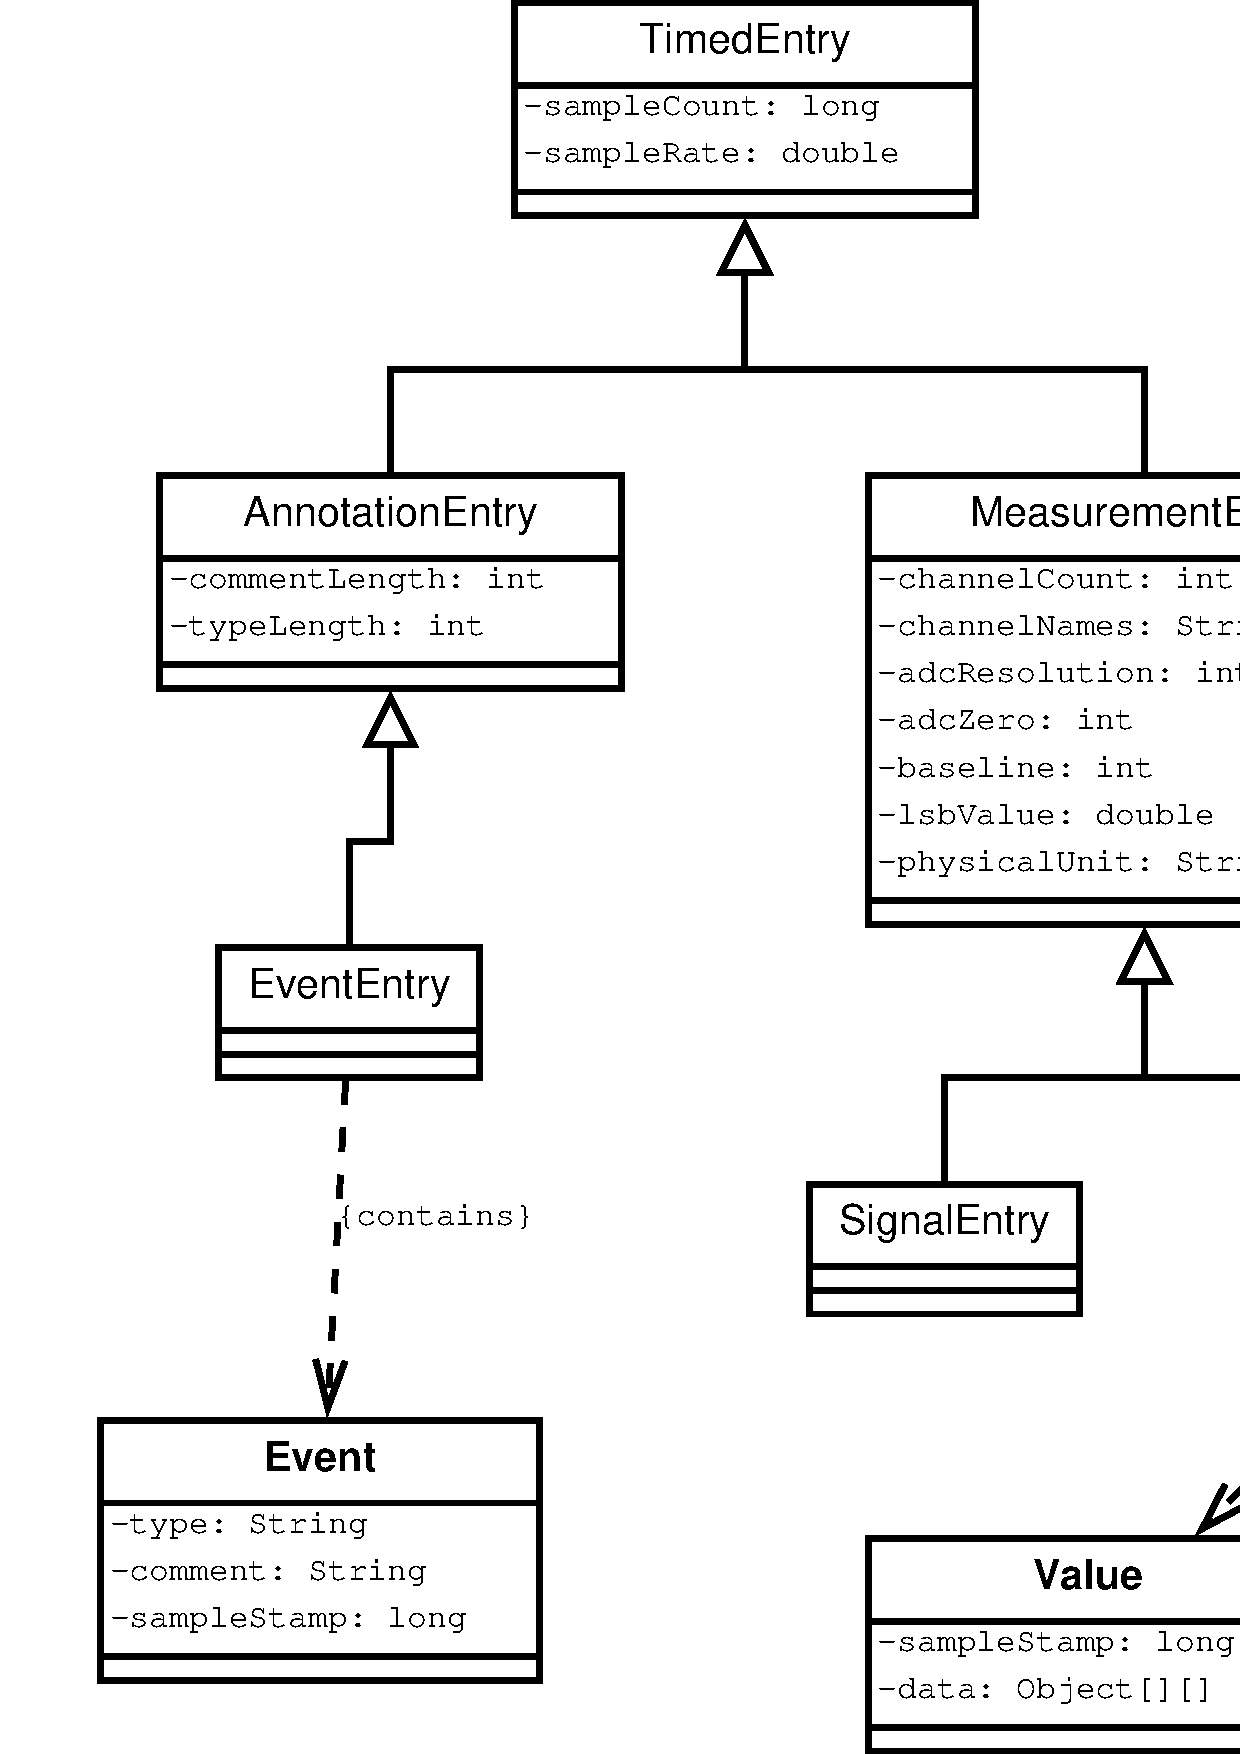
\includegraphics[width=\textwidth]{bilder/unisens_interface.png}
\caption{Klassen\"ubersicht der von Unisens definierten Schnittstellen}
\label{pic:unisens_interface}
\end{figure}

Die Zeitpunkte von Ereignisdaten und Einzelwertdaten werden \"uber eine virtuelle Abtastrate bestimmt.
Der Zeitpunkt eins jeden \emph{Event}- oder \emph{Value}-Eintrags ist als ganzzahlige Samplenummer dieser Abtastrate gespeichert.
Die Zeit eines Ereignisses, relativ zum Messbeginn, errechnet sich somit $Zeitpunkt = {Samplenummer \over Abtastrate}$.
M\"ochte man die M\"oglichkeit Ereignisse f\"ur jeden beliebigen Datenpunkt eines Datensatzes zuordnen zu k\"onnen, dann muss die virtuelle Abtastrate als das kleinste gemeinsame Vielfache aller vorhandenen Abtastraten gew\"ahlt werden.

...

%% EOF %%%%%%%%%%%%%%%%%%%%%%%%%%%%%%%%%%%%%%%%%%%%%%%%%%%%%%

\chapter{Vorbetrachtungen}

\section{Softwareentwurf}

Theorie zu Softwareentwurf

\section{Anwendungsf"alle}

Um eine Anforderungsliste an die zu erstellende Software ausarbeiten zu k"onnen, soll zun"achst eine Liste von Anwendungsf"allen ausgearbeitet werden.
Aus der Liste h"aufiger Arbeitsabl"aufe und typischer Aufgabenstellungen wird ersichtlich, was der Nutzer von der Software erwartet.
Mithilfe dieser Erwartungen k"onnen im Anschluss die Anforderungen an das Programm formuliert und festgelegt werden.
% besonderheiten/merkmale der zu ueberpruefenden signale
% typische aufgabenstellungen
% haeufige arbeitsablaeufe

% enumerate auf a), b), usw aendern
\renewcommand{\theenumi}{\alph{enumi}}
\renewcommand{\labelenumi}{\theenumi )}
% und los geht's
Der Anwender m"ochte ...
\begin{enumerate}
	\item einen Datensatzes laden.
		  Dieser Datensatz umfasst mehrere (Bio-) Signale die sowohl mit einer konstanten Abtastrate erfasst wurden als auch Signale die nicht zu "aquidistanten Zeitpunkten abgetastet wurden.
	\item einen geladenen Datensatz mit allen "Anderungen speichern.
		  Hierbei sollen auch Einstellungen gespeichert werden, die die optische Pr"asentation wiederspiegeln.
	\item sich Informationen zu dem geladenen Datensatz und seinen beinhalteten Signalen anzeigen lassen und ver"andern.
	\item bestimmte Signale des Datensatzes ausw"ahlen und sich diese in ihrem Verlauf anzeigen lassen (Signalansicht).
		  Hierbei m"ochte er Bildschirmgr"o\ss e der einzelnen Ansichten ver"andern.
	\item die Signalansicht bez"uglich der Zeit- und der Amplitudenachse vergr"o\ss ern und verkleinern k"onnen (Zoomen).
		  Entlang der Zeitachse m"ochte er sie verschieben k"onnen (Scrollen).
		  Signaleverl"aufe die parallel aufgenommen wurden, sollen auch zusammen gescrollt werden.
	\item in einer Signalansicht mehrere Signale mit denselben Achsen darstellen lassen.
		  Beispielsweise um ein Roh- und ein verarbeitetes Signal miteinander vergleichen zu k"onnen.
	\item einen Amplitudenbereich eines Signals optisch hervorheben.
	\item einzelne Zeitpunkte im Signalverlauf mit einer Markierung versehen und kommentieren.
		  Diese Markierung kann sowohl f"ur ein bestimmtes Signal gelten, aber auch f"ur alle Signale des Datensatzes.
	\item einen Zeitabschnitt markieren. Die Markierung der Abschnitte soll analog zur Markierung von Zeitpunkten erfolgen.
	\item die Markierungen ver"andern (zeitlich verschieben, umbennen) oder l"oschen.
	\item Markierungen gemeinsam mit dem Datensatz aber auch unabh"angig vom Datensatz abspeichern.
\end{enumerate}

\section{Anforderungen}

Aus den oben genannten Anwendungsf"allen ergeben sich die folgenden Anforderungen an das Programm.
Das Programm ...
\renewcommand{\theenumi}{\Alph{enumi}}
\renewcommand{\labelenumi}{\theenumi )}
\newcommand{\AF}[1]{\item \label{AF:#1}}
\begin{enumerate}
	\AF{gui} muss eine grafische Benutzeroberfl"ache besitzen.
	\AF{datensatz} muss ein Datensatzformat unterst"utzen, das "aquidistant und nicht "aquidistante abgetastete Signale speichern kann.
	\AF{datenmanagement} soll in der Lage sein, Daten aus einem Datensatz zu laden.
						 Dem Nutzer muss es erm"oglicht werden, diese Signaldaten aus einer "Ubersicht auszuw"ahlen und in Diagrammen darstellen zu lassen.
						 Ferner muss der Benutzer eine M"oglichkeit haben, sich allgemeine Informationen des Datensatzes anzeigen zu lassen.
	\AF{diagramm} muss in der Lage sein, die Signalverl"aufe sowohl einzeln in einem Diagramm daszustellen, aber auch mehrere verschieden Signalverl"aufe in ein und demselben Diagramm zu visualisieren.
				  Diese Signalansichten sollten in ihrer Darstellungsgr"o\ss e durch den Nutzer ver"anderbar sein.
	\AF{ansicht} soll dem Benutzer erm"oglichen, seine Signalansicht frei "`bewegen"' zu k"onnen.
				 Es muss eine Vergr"o\ss erung und Verkleinerung bez"uglich der Abszissen- und der Ordinatenachse unterst"utzen.
				 Zus"atzlich ist die F"ahigkeit des Verschiebens der Ansicht gefordert.
				 Dabei sollen mehrere Diagramme gleichzeitig Verschoben werden k"onnen.
	\AF{amplitudenmarkierung} muss in der Lage sein einen Amplitudenbreich ein oder mehrerer Signalansichten optisch hervorzuheben.
	\AF{annotationen} soll dem Nutzer ein Werkzeug zur Verf"ugung stellen, das ihm erlaubt Datenpunkte zu annotieren.
					  Diese Annotationen sollen optisch in den Signalansichten ersichtlich sein und mit einem Kommentar versehen werden k"onnen.
					  Neben der Annotation einzelner Datenpunkte, soll auch die Markierung von Signalbereichen unterst"utzt werden.
					  Ferner ist gefordert, dass vorhandene Annotationen ver"anderbar sind.
	\AF{io} muss "Anderungen an den Signalen selbst und den Annotationen speichern k"onnen.
			Annotationen m"ussen unabh"angig von anderen Signalen gespeichert werden k"onnen.
			Insbesondere d"urfen Annotationen sich nicht ver"andern, wenn sich das Ursprungssignal ver"andert oder nicht mehr vorhanden ist.
	\AF{einstellungen} soll interne Einstellungen abspeichern und von einer Sitzung zur n"achsten "ubernehmen.
					   Optionen bez"uglich der Darstellung von Signalen sollen in dem Datensatz mit abgespeichert werden k"onnen.
\end{enumerate}

Die in der Aufgabenstellung geforderte Ausbauf"ahigkeit der Programms ist nicht durch die Anwendungsf"alle abgedeckt.
Daher wird die folgenden Anforderung nur auf Basis der Aufgabenstellung formuliert:
%Die folgende Anforderung l"asst sich nicht aus den Anwendungsf"allen erschlie\ss en, das die Erweiterbarkeit eine Forderung von zuk"unftigen Entwicklern ist und nicht die der Anwender.
%Um aber die Ausbauf"ahigkeit des Programms zu erm"oglichen, muss es 
\begin{enumerate}[resume]
	\AF{signalverarbeitung} Das Programm soll dem Benutzer erm"oglichen eine Signalverarbeitungsmethode auf ein gew"ahltes Biosignal anwenden zu k"onnen.
							Dabei muss das Originalsignal unver"andert bleiben.
							Der bearbeitete Signalverlauf kann als eigenes Signal im Datensatz abgespeichert werden.
							Die Implementierung dieser Anforderung soll beispielhaft f"ur zuk"unftige Entwickler erfolgen um die Erweiterbarkeit zu gew"ahrleisten.
\end{enumerate}

\section{Testszenarien}

In der Softwareentwickluin

Um das Programm auf seine Funktionsf"ahigkeit zu "uberpr"ufen sollen in diesem Abschnitt Tests ausgearbeitet werden.
Sie erm"oglihcen es das Progrmam zu testen und auf seine funktionf"ahigkeit zu "uberpr"ufen.
Daher brauchen wir ein paar Testszenarien f"ur die FUnktionspr"ufung des F"ahigkeits"uberpr"ufungsroutinendingens.

% Szenarien aus der Anforderungsliste abgeleitet

%% EOF %%%%%%%%%%%%%%%%%%%%%%%%%%%%%%%%%%%%%%%%%%%%%%%%%%%%%%

\chapter{Spezifikation der Programmfunktionalit"at}
\label{chap:spezifikation}

Die Spezifikation der Software ist in dieser Arbeit in zwei Etappen aufgeteilt:
\begin{itemize}
	\item Aufstellen von Anwendungsszenarien
	\item Ableitung der notwendigen Anforderungen
\end{itemize}
Dabei ist das Ziel eine Liste mit konkreten Anforderungen an das zu erstellende Programm.
Das Aufstellen der Anwendungsszenarien dient einerseits dem Entwickler einen "Uberblick "uber die Gesamtproblematik zu erhalten.
Zus"atzlich dazu wird ersichtlich, welche Arbeitsschritte notwendig sind und wie diese zeitlich zu einander ausgef"uhrt werden.
Damit wird die vom Benutzer beabsichtigte Aktion in seine fundamentalen Bestandteile aufgeteilt.
Diese Bestandteile sind somit Funktionen die das Programm bereit stellen muss.
Es sind die zu erf"ullenden Anforderungen.

\section{Anwendungsszenarien}
\label{chap:anwendungsszenarien}

%In diesem und dem folgendem Abschnitt soll die zu erstellende Software genauer spezifiziert werden.
%In diesem und dem folgendem Abschnitt soll die Softwarespezifikation im Entwicklungsprozess beschrieben und ausgearbeitet werden.

Der erste Schritt stellt das Ausarbeiten von Szenarien dar, die eine Beschreibung eines Merkmals des Programmes aus Sicht des Anwenders ist.
%Dazu soll zun"achst eine Liste von Anwendungsf"allen ausgearbeitet werden.
%Um eine Anforderungsliste an die zu erstellende Software ausarbeiten zu k"onnen, soll zun"achst eine Liste von Anwendungsf"allen ausgearbeitet werden.
Aufgrund dieser informellen Beschreibungen h"aufiger Arbeitsabl"aufe und typischer Aufgabenstellungen wird eine "Ubersicht gewonnen, was die zu erstellende Software leisten soll und der Nutzer erwartet.
%Aus der Liste h"aufiger Arbeitsabl"aufe und typischer Aufgabenstellungen wird ersichtlich, was der Nutzer von der Software erwartet.
Mithilfe dieser Erwartungen k"onnen im Anschluss die funktionalen Anforderungen an das Programm formuliert und festgelegt werden.
Das Ergebnis ist somit die Beschreibung des notwendigen (Software-) Systemumfangs und der zu implementierenden Arbeitsprozesse.
% besonderheiten/merkmale der zu ueberpruefenden signale
% typische aufgabenstellungen
% haeufige arbeitsablaeufe

% enumerate auf a), b), usw aendern
\renewcommand{\theenumi}{\alph{enumi}}
\renewcommand{\labelenumi}{\theenumi )}
% und los geht's
Der Anwender m"ochte ...
\begin{enumerate}
	\item einen Datensatzes laden.
		  Dieser Datensatz umfasst mehrere (Bio-) Signale die sowohl mit einer konstanten Abtastrate erfasst wurden als auch Signale die nicht zu "aquidistanten Zeitpunkten abgetastet wurden.
	\item einen geladenen Datensatz mit allen "Anderungen speichern.
		  Hierbei sollen auch Einstellungen gespeichert werden, die die optische Pr"asentation wiederspiegeln.
	\item sich Informationen zu dem geladenen Datensatz und seinen beinhalteten Signalen anzeigen lassen und ver"andern.
	\item bestimmte Signale des Datensatzes ausw"ahlen und sich diese in ihrem Verlauf anzeigen lassen (Signalansicht).
		  Hierbei m"ochte er Bildschirmgr"o\ss e der einzelnen Ansichten ver"andern.
	\item die Signalansicht bez"uglich der Zeit- und der Amplitudenachse vergr"o\ss ern und verkleinern k"onnen (Zoomen).
		  Entlang der Zeitachse m"ochte er sie verschieben k"onnen (Scrollen).
		  Signaleverl"aufe die parallel aufgenommen wurden, sollen auch zusammen gescrollt werden.
	\item in einer Signalansicht mehrere Signale mit denselben Achsen darstellen lassen.
		  Beispielsweise um ein Roh- und ein verarbeitetes Signal miteinander vergleichen zu k"onnen.
	\item einen Amplitudenbereich eines Signals optisch hervorheben.
	\item einzelne Zeitpunkte im Signalverlauf mit einer Markierung versehen und kommentieren.
		  Diese Markierung kann sowohl f"ur ein bestimmtes Signal gelten, aber auch f"ur alle Signale des Datensatzes.
	\item einen Zeitabschnitt markieren. Die Markierung der Abschnitte soll analog zur Markierung von Zeitpunkten erfolgen.
	\item die Markierungen ver"andern (zeitlich verschieben, umbennen) oder l"oschen.
	\item Markierungen gemeinsam mit dem Datensatz aber auch unabh"angig vom Datensatz abspeichern.
\end{enumerate}

\section{Anforderungen an das Programm}
\label{chap:anforderungen}

Mithilfe der oben beschriebenen Anwendungsszenarien kann daraus die konkrete Funktionalit"at der Software definiert werden.
Diese Definition erfolgt durch die Bestimmung konkreter Anforderungen an das Programm.
Dabei beschreiben die Anforderungen die konkret umzusetzenden Funktionen und Arbeitswerkzeuge.
Zus"atzlich wird die in Kapitel \ref{chap:anforderungsvalidierung} beschriebene Validierung der Software die in diesem Abschnitt ausgearbeiteten Definitionen als Grundlage nehmen um das erstellte Programm zu "uberpr"ufen und zu bewerten.

%Aus den oben genannten Anwendungsf"allen ergeben sich die folgenden Anforderungen an das Programm.
Die folgende List von zu erf"ullenden Anforderungen ergibt sich aus den oben beschreibenen Anwendungsszenarien.
Wenn mehrere Einzelanforderungen in einer Beschreibung enthalten sind, sind diese mit einer Ziffer in Klammern markiert.
Das Programm ...
\renewcommand{\theenumi}{\Alph{enumi}}
\renewcommand{\labelenumi}{\theenumi )}
\newcommand{\AF}[1]{\item \label{AF:#1}}
\begin{enumerate}
	\AF{gui} muss eine grafische Benutzeroberfl"ache besitzen.
	\AF{datensatz} muss ein Datensatzformat unterst"utzen, das "aquidistant (1) und nicht "aquidistante (2) abgetastete Signale speichern kann.
	\AF{datenmanagement} soll in der Lage sein, Daten aus einem Datensatz zu laden (1).
						 Dem Nutzer muss es erm"oglicht werden, diese Signaldaten aus einer "Ubersicht auszuw"ahlen (2) und in Diagrammen darstellen zu lassen.
	\AF{dateninformation} muss dem Nutzer die M"oglichkeit bieten allgemeine Informationen sowohl "uber den Datensatz (1) als auch "uber die enthaltenen Daten (2) anzuzeigen.
	\AF{diagramm} muss in der Lage sein, die Signalverl"aufe sowohl einzeln (1) in einem Diagramm darzustellen, aber auch mehrere verschieden Signalverl"aufe (2) in ein und demselben Diagramm zu visualisieren.
				  Diese Signalansichten sollten in ihrer Darstellungsgr"o\ss e durch den Nutzer ver"anderbar sein (3).
	\AF{ansicht} soll dem Benutzer erm"oglichen, seine Signalansicht frei "`bewegen"' zu k"onnen.
				 Es muss eine Vergr"o\ss erung und Verkleinerung bez"uglich der Abszissen- und der Ordinatenachse unterst"utzen (1).
				 Zus"atzlich ist die F"ahigkeit des Verschiebens der Ansicht gefordert (2).
				 Dabei sollen mehrere Diagramme gleichzeitig Verschoben werden k"onnen (3).
	\AF{amplitudenmarkierung} muss in der Lage sein einen Amplitudenbereich ein oder mehrerer Signalansichten optisch hervorzuheben.
	\AF{annotationen} soll dem Nutzer ein Werkzeug zur Verf"ugung stellen, das ihm erlaubt Datenpunkte zu annotieren (1).
					  Diese Annotationen sollen optisch in den Signalansichten ersichtlich sein (2) und mit einem Kommentar versehen werden k"onnen (3).
				  	  Ferner ist gefordert, dass vorhandene Annotationen ver"anderbar sind (4).
	\AF{breichsannotation} soll neben der Annotation einzelner Datenpunkte auch die Markierung von Signalbereichen unterst"utzt werden.
	\AF{io} muss "Anderungen an den Signalen selbst (1) und den Annotationen (2) speichern k"onnen.
			Annotationen m"ussen unabh"angig von Signalen gespeichert werden k"onnen (3).
			Insbesondere d"urfen Annotationen sich nicht ver"andern, wenn sich das Ursprungssignal ver"andert oder nicht mehr vorhanden ist (4).
	\AF{einstellungen} soll interne Einstellungen abspeichern und von einer Sitzung zur n"achsten "ubernehmen (1).
					   Optionen bez"uglich der Darstellung von Signalen sollen in dem Datensatz mit abgespeichert werden k"onnen (2).
\end{enumerate}

Die in der Aufgabenstellung geforderte Ausbauf"ahigkeit der Programms ist nicht durch die Anwendungsszenarien abgedeckt werden.
Hierbei handelt es sich um eine nichtfunktionale Anforderung an das Programm.
Daher wird die folgenden Anforderung nur auf Basis der Aufgabenstellung formuliert und nicht aufgrund der Erwartungshaltung des Benutzers:
%Die folgende Anforderung l"asst sich nicht aus den Anwendungsf"allen erschlie\ss en, das die Erweiterbarkeit eine Forderung von zuk"unftigen Entwicklern ist und nicht die der Anwender.
%Um aber die Ausbauf"ahigkeit des Programms zu erm"oglichen, muss es 
\begin{enumerate}[resume]
	\AF{signalverarbeitung} Das Programm soll dem Benutzer erm"oglichen eine Signalverarbeitungsmethode auf ein gew"ahltes Biosignal anwenden zu k"onnen (1).
							Dabei muss das Originalsignal unver"andert bleiben (2).
							Der bearbeitete Signalverlauf kann als eigenes Signal im Datensatz abgespeichert werden (3).
							Die Implementierung dieser Anforderung soll beispielhaft f"ur zuk"unftige Entwickler erfolgen um die Erweiterbarkeit zu gew"ahrleisten.
\end{enumerate}

\section{Testszenarien}
\label{chap:testszenarien}

In diesem Abschnitt sollen Szenarien heraus gearbeitet werden, mit denen die Software am Ende der Implementierung validiert werden kann.
Dabei soll die oben geforderte Funktionalit"at anhand der Behandlung von Biosignalen "uberpr"uft werden.

Folgend sollen die Testszenarien beschrieben werden die zur Validierung der Software durchgef"uhrt werden sollen.
Die Ausgangsbedingung ist eine das einfache Starten des Programmes.
Somit soll der erste, nicht jeweils explizit genannte Schritt sein, das Programm zu starten.
Abgeschlossen wird jedes Testszenario mit dem Speichern der geladenen Daten.
\begin{description}
\item[Testszenario 1] Der Benutzer l"adt einen Datensatz abdominaler \ac{EKG}-Daten mit sieben Aufnahmekan"alen.
					  Zus"atzlich sind noch die approximierten \ac{EKG}-Signale des Fetus sowie der Mutter im Datensatz gespeichert.
					  Der Benutzer l"asst sich alle verf"ugbaren Informationen zu dem geladenem Datensatz anzeigen.
					  Anschlie\ss end l"asst er sich einen Kanal sowohl des Rohsignals als auch der beiden abgeleiteten Signale jeweils in einer eigenen Ansicht anzeigen.
					  Er verschafft sich durch eine geringe Zoomstufe einen "Uberblick "uber die Signalverl"aufe.
					  Der Benutzer zoomt auf interessante Bereiche der Aufnahme herein und vergr"o\ss ert die Ansicht der Einzelsignale.
					  Er schlie{\ss}t die Ansicht des Rohsignals.
					  Der Benutzer markiert in zwei unterschiedlichen, neu zu erstellenden Annotationskan"alen die QRS-Komplexe der Mutter, sowie des Fetus ("uber mindestens f"unf Minuten des Signalverlaufs).
					  Zur "Uberpr"ufung der Annotationen l"asst er sich alle Signale und die gemachten Annotationen in einer Signalansicht darstellen.
\item[Testszenario 2] Der Benutzer l"adt den im Testszenario abgespeicherten Datensatz wieder in das Programm.
					  Er "uberpr"uft ob die Ansichten und die Einstellungen aus dem ersten Testszenario "ubernommen wurden.
					  Der Benutzer speichert die Einstellungen der Signalansichten.
					  Er w"ahlt f"unf beliebige Annotationen aus versieht diese mit Kommentaren.
					  Der Benutzer l"oscht jede zweite Annotation des fetalen QRS-Komplexes.
					  Weiterhin soll er mindestens 10 Zeitbereiche markieren, wobei es auch zu "Uberschneidungen diese Bereiche kommen soll.
					  Er l"adt die zuvor gespeicherten Einstellungen und "uberpr"uft ob diese richtig geladen wurden.
\item[Testszenario 3] Der Benutzer l"adt den Bearbeiteten Datensatz aus dem zweiten Testszenario.
					  Er entfernt die Kan"ale der approximierten \ac{EKG}-Verl"aufe aus dem Datensatz.
					  Der Benutzer "uberpr"uft die gemachten Annotationen mithilfe des Rohsignals.
\item[Testszenario 4] Der Benutzer l"adt einen Datensatz mit \ac{EKG}-und \ac{PPG}-Signalen.
					  Er w"ahlt \ac{PPG} und \ac{EKG} Kan"ale und zeigt sie sich in einer Ansicht an.
					  Der Benutzer verschafft sich eine "Ubersicht durch eine geringe Zoomstufe "uber die Signalverl"aufe.
					  Der Benutzer markiert einen Amplitudenbereich im \ac{PPG}-Signal.
					  Er wendet eine Filterfunktion auf das \ac{EKG}-Signal an und speichert das Ergebnis im Datensatz ab.
					  Er kontrolliert die Informationen des ver"anderten Signals.
					  Der Nutzer entfernt das Original-\ac{EKG}-Signal aus dem Datensatz.
\item[Testszenario 5] Der Benutzer l"adt den Datensatz aus dem viertem Testszenario.
					  Er kontrolliert dabei die Einstellungen der Ansichten darauf, ob sie aus dem Szenario 4 "ubernommen wurden.
					  Er annotiert die QRS-Komplexe des gefiltertem \ac{EKG}-Signals f"ur mindestens f"unf Minuten des Signalverlaufs.
					  Der Benutzer wendet eine weitere Filterfunktion auf das bereits gefilterte Signal an und speichert das Ergebnis erneut im Datensatz ab.
					  Er kontrolliert die Annotationen mit dem erneut gefiltertem Signal.
\end{description}

\begin{table}[htb]
\caption[Abdeckung der Anforderungen durch die Testszenarien]{Abdeckung der Anforderungen durch die Testszenarien (TS)}
\label{tab:anforderungs_abdeckung}
\centering
\begin{tabular}{|r|c|c|c|c|c|c|c|c|c|c|c|c|c|c|c|c|c|}
	\cline{2-17}
	\multicolumn{1}{r|}{} & \multicolumn{16}{|c|}{Anforderung} \\ \cline{2-17}
	\multicolumn{1}{r|}{} & A & B1 & B2 & C1 & C2 & D1 & D2 & E1 & E2 & E3 & F1 & F2 & F3 & G & H1 & H2\\ \hline
	TS 1 & \Checkmark & \Checkmark &  & \Checkmark & \Checkmark & \Checkmark & \Checkmark & \Checkmark & \Checkmark & \Checkmark & \Checkmark & \Checkmark & \Checkmark & & \Checkmark & \Checkmark \\ \hline
	TS 2 & \Checkmark & \Checkmark & & \Checkmark & \Checkmark & & & \Checkmark & & & \Checkmark & \Checkmark & \Checkmark & & & \Checkmark \\ \hline
	TS 3 & \Checkmark & \Checkmark & & \Checkmark & \Checkmark & & & \Checkmark & & & \Checkmark & & & & & \Checkmark \\ \hline
	TS 4 & \Checkmark & \Checkmark & \Checkmark & \Checkmark & \Checkmark & & \Checkmark & \Checkmark & & \Checkmark & \Checkmark & \Checkmark & \Checkmark & \Checkmark & & \\ \hline
	TS 5 & \Checkmark & \Checkmark & \Checkmark & \Checkmark & \Checkmark & & & \Checkmark & & & \Checkmark & \Checkmark & \Checkmark & \Checkmark & & \Checkmark \\ \hline
\end{tabular}

\vspace{2ex}

\begin{tabular}{|r|c|c|c|c|c|c|c|c|c|c|c|c|c|}
	\cline{2-13}
	\multicolumn{1}{r|}{} & \multicolumn{12}{|c|}{Anforderung} \\ \cline{2-13}
	\multicolumn{1}{r|}{} & H3 & H4 & I & J1 & J2 & J3 & J4 & K1 & K2 & L1 & L2 & L3 \\ \hline
	TS 1 & & & & & \Checkmark & & & & & & & \\ \hline
	TS 2 & \Checkmark & \Checkmark & \Checkmark & & \Checkmark & & & \Checkmark & \Checkmark & & & \\ \hline
	TS 3 & & & & & & \Checkmark & \Checkmark & & \Checkmark & & & \\ \hline
	TS 4 & & & & \Checkmark & & & & & & \Checkmark & \Checkmark & \Checkmark \\ \hline
	TS 5 & & & & \Checkmark & \Checkmark & \Checkmark & \Checkmark & \Checkmark & \Checkmark & \Checkmark & \Checkmark & \Checkmark \\ \hline
\end{tabular}
\end{table}

In \ac{tab} \ref{tab:anforderungs_abdeckung} ist "ubersichtlich aufgelistet welche der Anforderungen durch die Testszenarien abgedeckt sind.
Es ist erkenntlich, dass alle Anforderungen mindestens durch ein Testszenario "uberpr"uft wird.
Durch das Bestehen der Testszenarien wird gezeigt, dass das Programm die Erwartungen des Nutzers erf"ullt.

Das Testen der Funktionalit"at mittels bestimmter Biosignale sind aber nur spezielle Einzelf"alle.
Es kann durch sie nicht die absolute Fehlerfreiheit der Software gezeigt werden.
Um entstehende Fehler schon w"ahrend der Entwicklung abfangen und beheben zu k"onnen, wird die Software bzw. die einzelnen Programmteile auch schon einzeln daraufhin getestet, dass sie sich so verhalten, wie es der Programmierer vorgesehen hat.
Speziell wird auch das korekte Verhalten im Falle eines Fehlers "uberpr"uft.
Diese fortlaufenden funktionellen Test werden in den entsprechenden Abschnitten zu den einzelnen Programmkomponenten im Kapitel \ref{chap:entwurf} beschrieben.

%-- Implementierung und Fehlerbehebung
%-- konstant fortlaufender prozess
%-- komponenten test hier nicht abgebildet und beschrieben - sind schon durch inkrementelle entwicklung gef"ordert

\chapter{Programmentwurf}
\label{chap:entwurf}

In diesem Kapitel m"ochte der Autor die Entwicklung des Gesamtprogramms er"ortern.
Es wird ein "Uberblick "uber das umfassende Konzept des internen Aufbaus gegeben um anschlie\ss end auf die konkrete Umsetzung der einzelnen Bestandteile einzugehen.
Demzufolge sind die kommenden Abschnitte nach den Programmkomponenten gegliedert.
In jedem einzelnen Abschnitt wird auf drei Punkte eingegangen:
\begin{itemize}
	\item Grundlegende Idee und Designkonzept
	\item Implementierungsdetails
	\item Tests zur Verifikation der einzelnen Komponente
\end{itemize}
Es sei darauf hingewiesen, dass die eigentlichen Entwicklung und Implementierung nicht Komponentenweise, sondern nach entsprechenden Funktionalit"aten statt findet.
Das Einbinden einer bestimmten Funktionalit"at betrifft oft mehrere Komponenten und ihr Zusammenspiel, wodurch der Ausbau der einzelnen Bestandteile parallel geschieht.
Die Gliederung dieses Kapitels nach den Programmteilen dient jedeglich der "Ubersichtlichkeit.

\section{[WIP]"Uberblick "uber das Gesamtprogramm}

\begin{figure}[htb]
\centering
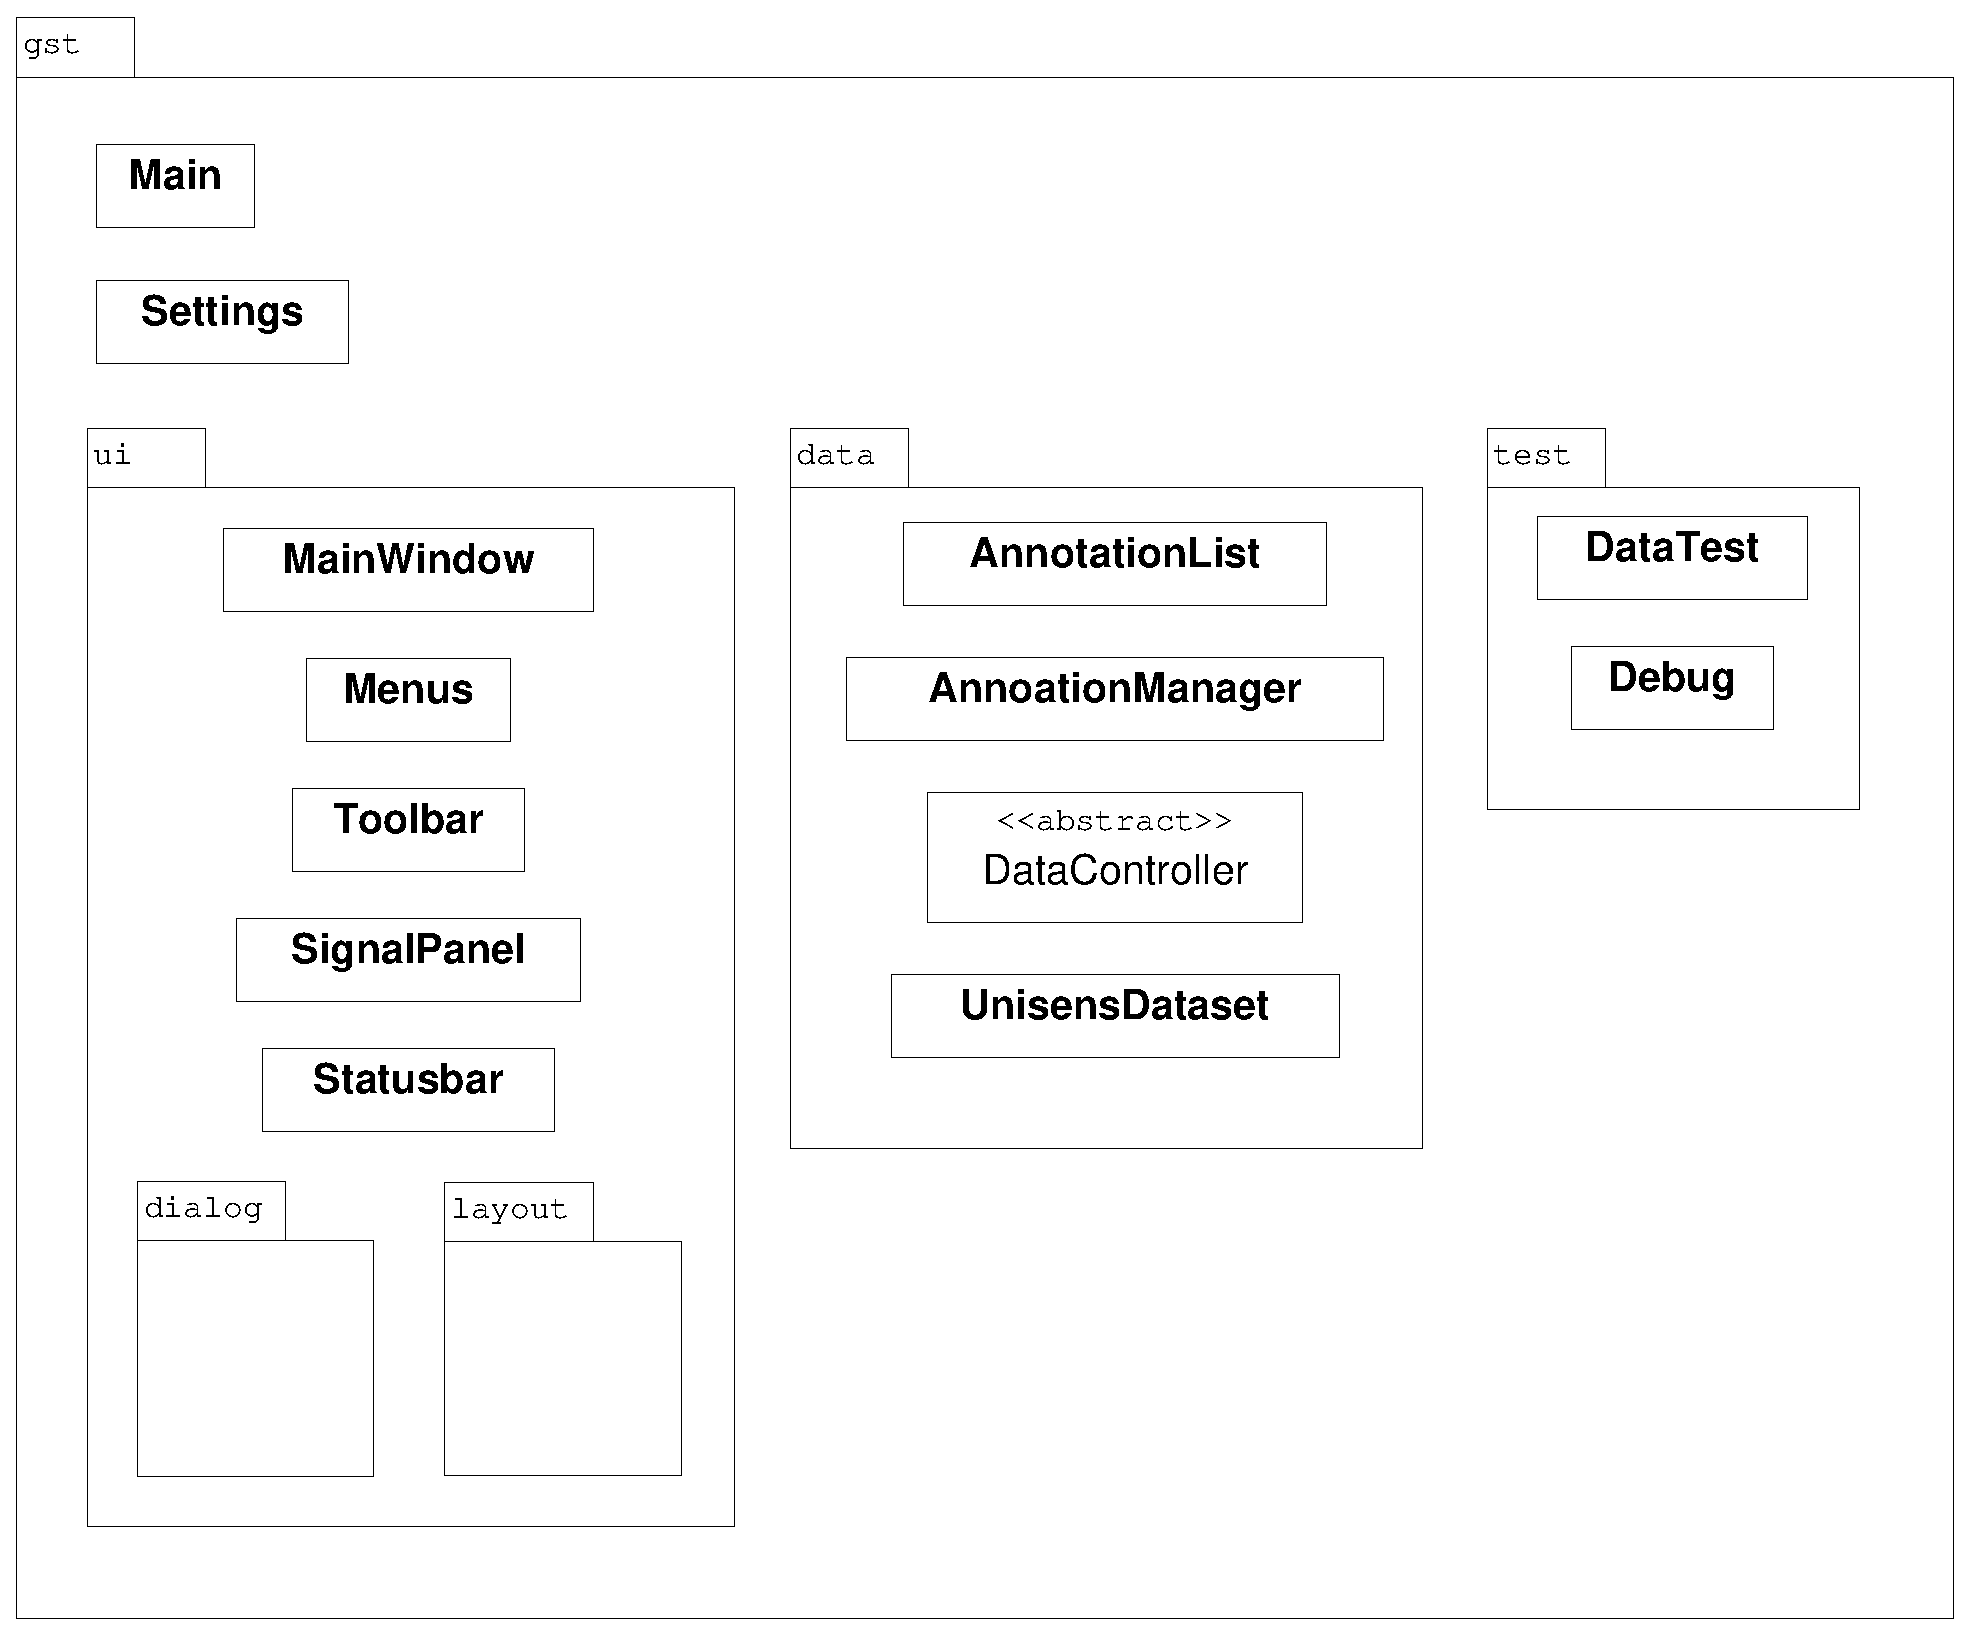
\includegraphics[width=0.9\textwidth]{bilder/prog_ubersicht.eps}
\caption[\ac{uml}-Paket-"Ubersicht der umgesetzten Software]{\ac{uml}-Paket-"Ubersicht der umgesetzten Software, nur wesentliche Klassen sind dargestellt}
\label{pic:paket_ubersicht}
\end{figure}

\begin{table}[hbt]
\centering
\caption[Paket- und Klassen"ubersicht]{Paket- und Klassen"ubersicht: Paketnamen sind in \texttt{True-Type} und Klassennamen in \textsf{serifenloser} Schriftart geschrieben}
\label{tab:klassenubersicht}
\textsf{
	\begin{tabular}{|llll|}
		\hline
		\texttt{gst} & Main &&\\ 
		    		 & Settings &&\\\hline
		\texttt{gst.}& \texttt{data} & AnnotationController &\\
					 &				 & AnnotationList &\\
					 &				 & AnnotationManager &\\
					 &				 & DataController &\\
					 &				 & SignalController &\\
					 &				 & UnisensDataset &\\
					 &				 & ValueController &\\\hline
		\texttt{gst.}& \texttt{test} & DataTest &\\
					 &				 & Debug &\\\hline
		\texttt{gst.}& \texttt{ui}	 & AnnotationSelectionDialog &\\
					 &				 & DataSelectionDialog &\\
					 &				 & MainWindow &\\
					 &				 & Menus &\\
					 &				 & NamedMouseAdapter &\\
					 &				 & Sidebar &\\
					 &				 & SignalOverview &\\
					 &				 & SignalPanel &\\
					 &				 & SignalView &\\
					 &				 & SignalViewFactory &\\
					 &				 & StatusBar &\\
					 &				 & Toolbar &\\\hline
		\texttt{gst.}& \texttt{ui.}	 & \texttt{dialog} & DatasetSelectionDialog\\
					 &				 &				   & EditEventDialog \\
					 &				 &				   & EnterFileNameDialog \\\hline
		\texttt{gst.}& \texttt{ui.}	 & \texttt{layout} & ComponentArrangement \\
					 &				 &				   & MultiSplit\\
					 &				 &				   & SignalPanelLayoutManager\\
					 &				 &				   & VerticalLayoutManager\\\hline
\end{tabular}
}
\end{table}

-- theoretische beschreibung des gesamtkonzeptes
-- komplette auflisten der subkomponenten in \tabref{klassenubersicht}
-- graphische "Ubersicht der Bestandteile siehe \picref{paket_ubersicht}

\section{Datenbehandlung}

Aufgrund der Vielfalt der genutzten Datenformate zur Speicherung von Biosignalen und der Nichtexistenz eines einheitlichen Standards \cite{Schlogl2009, Varri2001, Wang2010} muss ein Format gesucht werden, dass zur Behandlung von Datens"atzen im Rahmen dieser Arbeit geeignet ist.
Die Wahl des Datensatzformates st"utzt sich auf die vergleichende Untersuchung \cite{Schlogl2009} von Dr. Alois Schl"ogl der Technischen Universit"at Graz.
Das Unisens-Format besitzt eine Referenzimplementierung mit Programmierschnittstellen sowohl f"ur Matlab als auch f"ur Java und bietet f"ur diese Arbeit optimale Anwendungsvoraussetzungen.
Die Organisation "uber eine menschlich les- und editierbare Headerdatei ist gerade in der Entwicklung interessant.
Es kann ein Datensatz einfach und ohne Bearbeitungstools ver"andert und an die Bed"urfnisse angepasst werden.
Einer der Kritikpunkte nach \cite{Schlogl2009} ist, dass das Format aus mehreren Dateien besteht.
Da die Behandlung von Dateien und Verzeichnissen mit der aktuellen Software kaum noch Unterschiede f"ur den Anwender darstellt, ist nach Meinung des Autors dieser Punkt nicht von hoher Priorit"at.
Es bietet sogar die M"oglichkeit Daten direkt von Sensoren (bei bekannten technischen Parametern wie z.B. Abtastrate und -aufl"osung) direkt in einen Datensatz integriert werden k"onnen.
Zus"atzlich bietet das Format durch seine Definition eine gute Erweiterbarkeit.
Es kann somit an die neue Gegebenheiten und Voraussetzungen angepasst und optimiert werden.

%	-- menschlich editierbar (xml header)
%	-- verzeichnis vs eine datei ist vernachl"assigbar
%	-- reine sensordaten importierbar
%	-- implementierung vorhanden
%	-- f"ur matlab und java

\subsection{Unisens}

Das vom Forschungszentrum Informatik und Institut f"ur Technik der Informationsverarbeitung der Universit"at Karlsruhe entwickelte Datenformat Unisens dient der Speicherung und der Dokumentation von Sensordaten.
Unisens ist konzipiert, Daten verschiedener Sensoren innerhalb eines Datensatzes zu speichern.
Ein Datensatz ist im Dateisystem durch ein eigenes Verzeichnis und eine Headerdatei \verb|unisens.xml| hinterlegt.
In der Headerdatei werden alle Informationen "uber die Bestandteile des Datensatzes, deren Formatierung und ihre semantischen Zusammenh"ange gespeichert.
Messwerte eines Sensors werden "ublicherweise in einer Datendatei innerhalb des Datensatzverzeichnisses abgespeichert.
Eine solche Datendatei wird als \emph{Entry} in dem Datensatz bezeichnet.
Alle Metainformationen zu den Sensordaten werden in der Headerdatei abgspeichert, so dass die Datendateien selbst immer nur die reinen Messdaten enthalten.
Als m"ogliche Sensordaten werden sowohl kontinuierlich abgetastete Signale als auch ereignisorientierte Daten unterst"utzt.
Unisens unterscheidet zwischen vier Arten von Daten:
\begin{description}
	\item[Signale \emph{(Signal)}] \hfill \\
		Signale sind "aquidistant abgetastete, numerische Messdaten.
		Sie zeichnen sich durch eine beliebige aber konstante Abtastrate und Abtastaufl"osung aus.
		Zudem k"onnen Signale aus mehreren Kan"alen bestehen, die alle in ein und derselben Datei abgespeichert werden.
		Alle Kan"ale desselben Signals haben auch dieselbe Abtastrate und -aufl"osung.
	\item[Ereignisse \emph{(Event)}] \hfill \\
		Ereignisse sind diskrete Zeitpunkte die mit einer textlichen Beschreibung versehen sind. (z.B. Triggersignale)
		Sie zeichnen sich durch einen Zeitstempel und einer kurzen Beschreibung aus.
		Optional k"onnen noch Kommentare zu einem Ereignis hinzugef"ugt werden.
	\item[Einzelwerte \emph{(Value)}] \hfill \\
		Einzelwerte sind eine Kombination der beiden oben genannten Datenarten.
		Sie beinhalten numerische Werte die zu bestimmten Zeitpunkten aufgenommen wurden.
		Mit Einzelwerten ist es m"oglich Daten zu speichern, die nicht in festen Zeitintervallen gemessen werden.
	\item[Propriet"are Daten \emph{(Custom data)}] \hfill \\
		Mit dieser Art k"onnen anwendungsspezifisch Daten gespeichert werden, die durch die drei oben genannten Arten nicht erfasst werden k"onnen.
		So k"onnen beispielsweise schematische Darstellungen des Messaufbaus als Bilddateien oder Patienteakten in Form von Textdateien dem Datensatz hinzugef"ugt werden.
\end{description}
Eine detailiertere Beschreibung des Formates kann der offiziellen Dokumentation \cite{Ottenbacher2010} entnommen werden.

\subsubsection{Details der Referenzimplementierung}

In diesem Abschnitt wird kurz auf einige Details der Umsetzung des Unisens-Formates eingegangen.
Das Unisens-Paket ist in Java implementiert und wird unter der \emph{\ac{LGPL}} zur Verf"ugung gestellt.
Die bereit gestellte Bibliothek ist auf zwei Einzeldateien aufgeteilt: \verb|org.unisens.jar| und \verb|org.unisens.ri.jar|.
Bei der ersten Datei handelt es sich um die Definiton des Unisensformates und seiner Bestandteile als Javalassenstruktur.
Diese Definition erfolgt haupts"achlich als \emph{Interface}klassen und legt die Schnittstellen zwischen den einzelnen Bestandteilen fest.
Eine "Ubersicht der Klassenstruktur und der von au\ss en ersichtlichen Attribute ist in \picref{unisens_interface} auf Seite \pageref{pic:unisens_interface} dargestellt.
\begin{sidewaysfigure}
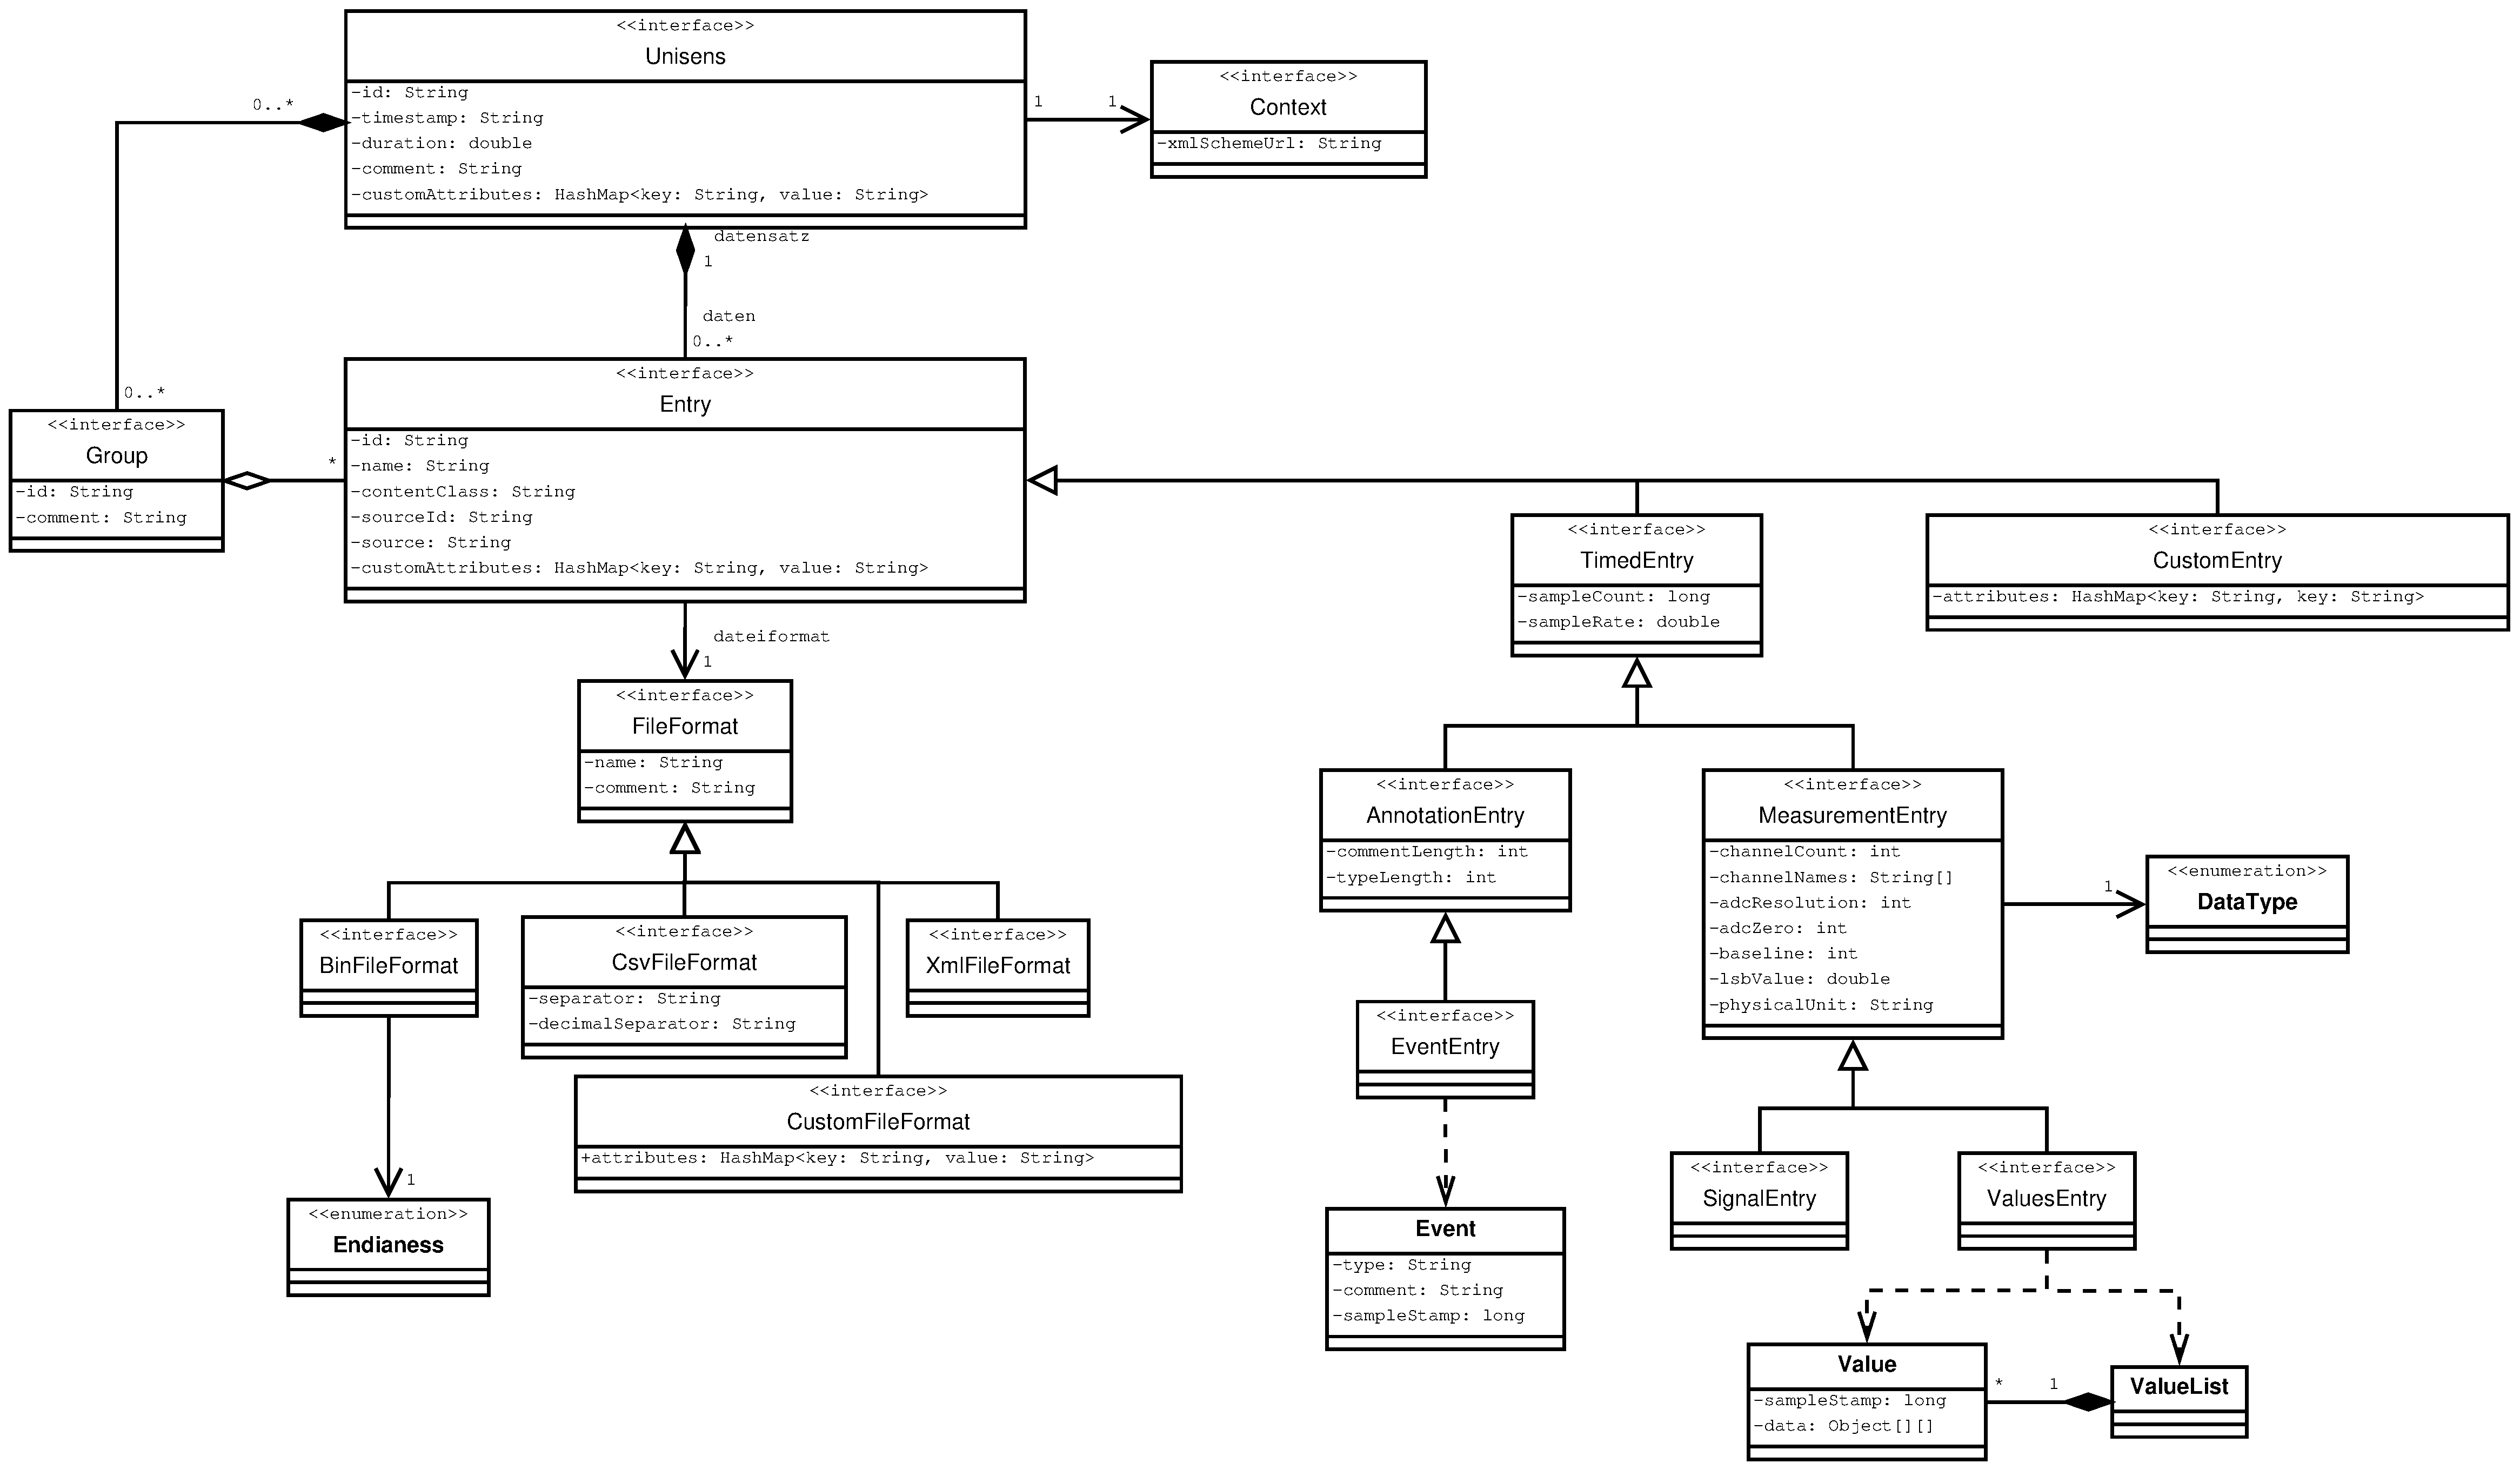
\includegraphics[width=\textwidth]{bilder/unisens_interface_.eps}
\caption{Klassen"ubersicht der von Unisens definierten Schnittstellen}
\label{pic:unisens_interface}
\end{sidewaysfigure}
Die vom Unisensformat unterst"utzten Signalarten sind auch in der Klassenstruktur in \tabref{unisens_signalklassen} erkennbar.
\begin{table}[h]
\centering
\begin{tabular}{|c|c|}
	\hline Signale & \verb|SignalEntry| \\
	\hline Ereignisse & \verb|EventEntry| \\
	\hline Einzelwerte & \verb|ValuesEntry| \\
	\hline Propriet"are Daten & \verb|CustomEntry| \\
	\hline
\end{tabular}
\caption{Signalarten und ihre repr"asentierenden Klassen}
\label{tab:unisens_signalklassen}
\end{table}

Aufgrund der Ableitung der Klassen \verb|EventEntry| und \verb|ValuesEntry| von \verb|TimedEntry| ist ersichtlich, dass die Zeitpunkte von Ereignisdaten und Einzelwertdaten "uber eine virtuelle Abtastrate bestimmt werden.
Der Zeitpunkt eines jeden \emph{Event}- oder \emph{Value}-Eintrags ist als ganzzahlige Samplenummer dieser Abtastrate gespeichert.
Die Zeit eines Ereignisses, relativ zum Messbeginn, errechnet sich somit $Zeitpunkt = {Samplenummer \over Abtastrate}$.
M"ochte man die M"oglichkeit Ereignisse f"ur jeden beliebigen Datenpunkt eines Datensatzes zuordnen zu k"onnen, dann muss die virtuelle Abtastrate als das kleinste gemeinsame Vielfache aller vorhandenen Abtastraten gew"ahlt werden.

Die Schnittstellendefinition des Unisensformats stellt nur Methoden zum Lesen und Anh"angen von Datenpunkten an den Datensatz bereit.
Somit wird ein Einf"ugen, L"oschen oder Ver"andern von Datenpunkten innerhalb eines Dateneintrags nicht unterst"utzt.
Sollen diese Funktionen vorhanden sein, so muss diese Funktionalit"at selbst implementiert werden.

Die eigentliche Umsetzung der Funktionalit"at ist in der zweiten Datei abgespeichert.
Im Folgenden soll sich der Begriff Referenzimplementierung auf diese funktionelle Umsetzung beziehen.
Die Klassen der Referenzimplementierung bestehen aus den Klassennamen der Schnittstellendefinition und dem Suffix "`Impl"' (z.B. Objekte die den Datensatz darstellen haben die Klasse \verb|UnisensImpl|).
Wenn man schon vorhandene Unisensdatens"atze benutzen m"ochte reicht es aus, die Schnittstellendefinition zu kennen und zu nutzen.
Sollen hingegen konkret Objekte erstellt werden, muss auf die Referenzimplementierung zur"uckgegriffen werden.

Durch einen Fehler in der Referenzimplementierung kann es vorkommen, dass beim Laden eines vorhandenen Unisensdatensatzes in dem Gruppen definiert sind eine \verb|NullPointerException| auftritt.
Insbesondere tritt dieser Fehler auf, wenn innerhalb der Headerdatei der Gruppeneintrag nicht hinter den Dateneintr"agen steht.

\subsection{Programminterne Datenstruktur}

\begin{figure}[htb]
\centering
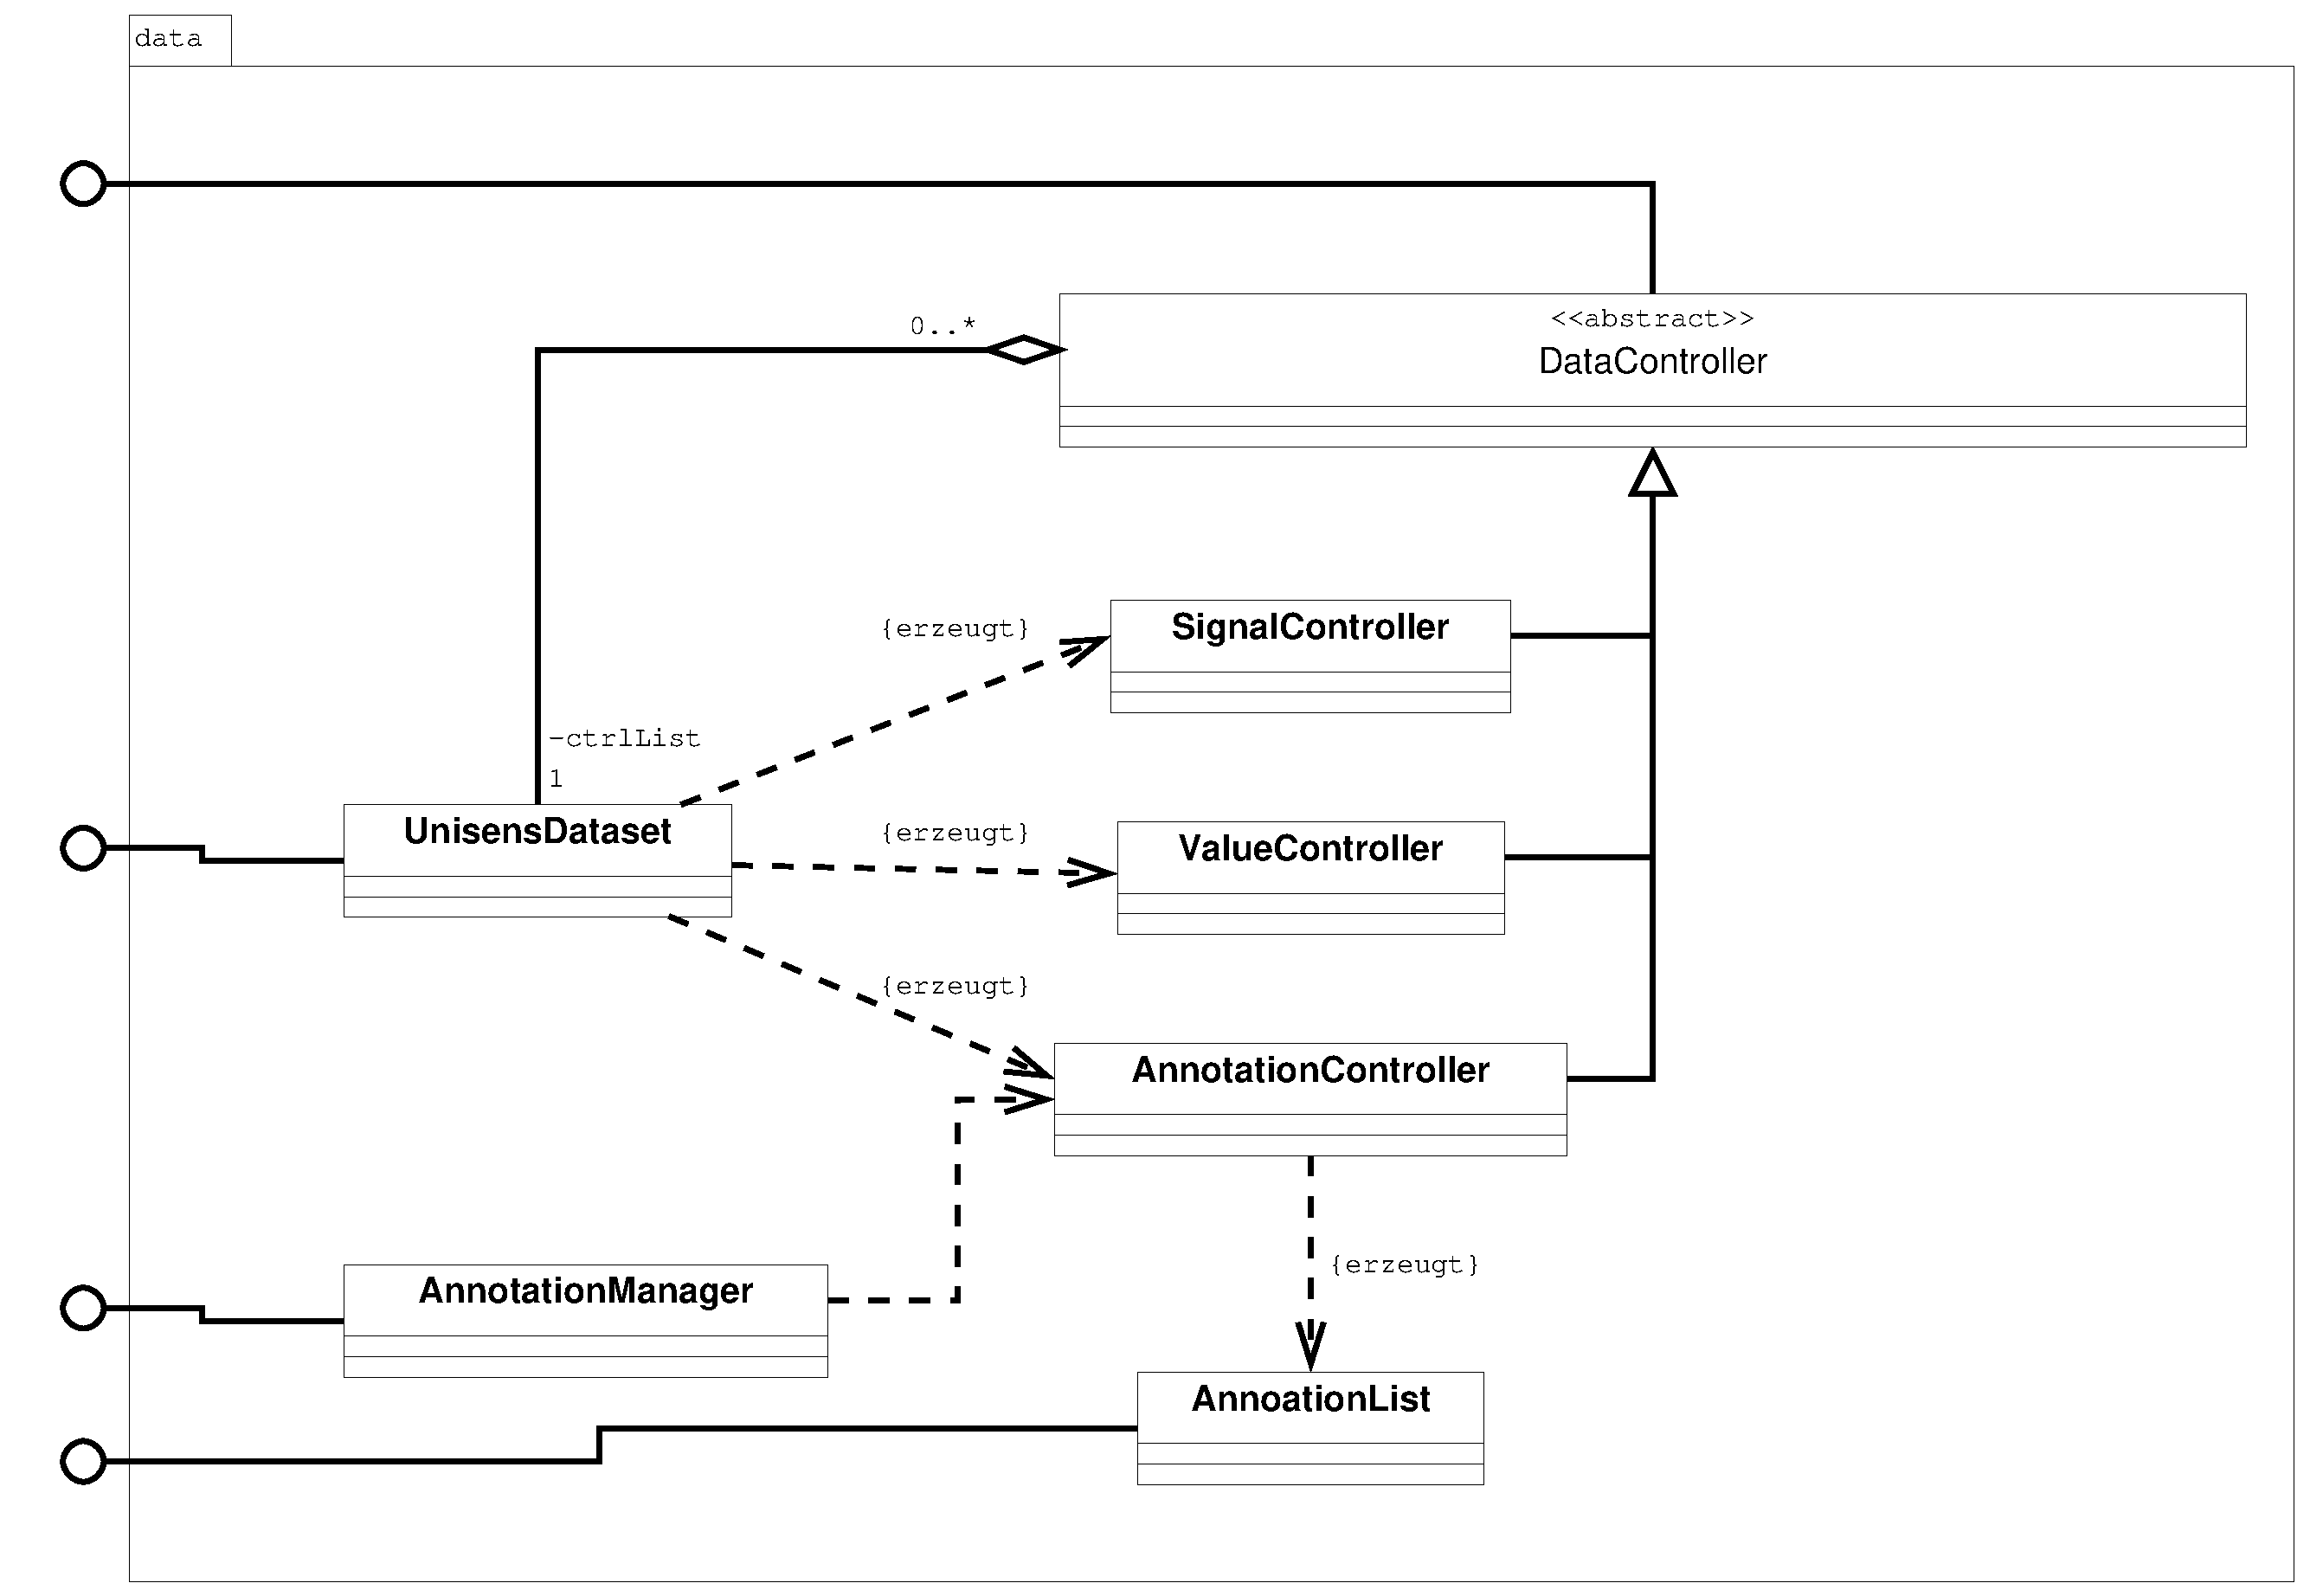
\includegraphics[width=0.9\textwidth]{bilder/prog_data_ubersicht.eps}
\caption[\ac{uml}-Diagramm des \texttt{data}-Paketes]{\ac{uml}-Diagramm des \texttt{data}-Paketes inklusive der bereitgestellten Schnittstellen}
\label{pic:data_package}
\end{figure}

Das Paket \verb|gst.data| ist die Schnittstelle der Programms zu dem gew"ahlten Datensatzformat Unisens.
Eine "Ubersicht des Paketes ist im \ac{uml}-Diagramm in \picref{data_package} dargestellt.
Dieses Paket erf"ullt zwei wesentliche Aufgaben:
\begin{itemize}
	\item Vereinheitlichung der Behandlung der unterschiedlichen Datenarten
	\item Abkapselung anderer Programmteile vom Datensatzformat
\end{itemize}

Die Vereinheitlichung ist notwendig, da Unisens die Daten in drei Arten gliedert: Signale, Werte und Ereignisse.
F"ur die Bearbeitung und Darstellung ist aber die Unterscheidung von Signalen und Werten nicht notwendig.
In beiden F"allen handelt es sich um numerische Werte die zu einem bestimmten Zeitpunkt aufgenommen wurden.
Somit sollen diese auch vom Programm gleichartig behandelt werden.
Daher erhalten alle Datenarten die abstrakte Klasse \verb|DataController| als Fassade.
Die jeweilge konkrete Implementierung ist in den drei abgeleiteten Klassen \verb|Signal-|, \verb|Value-| und \verb|AnnotationController| realisiert.
Neben der Vereinheitlichung der Schnittstelle zum Datensatz werden auch die Zugriffe auf die Daten vereinfacht.
Es werden notwendige Ausnahmebehandlungen (\emph{Exceptions}) durch die Klassen des \verb|data|-Paketes abgefangen und behandelt.
Darunter f"allt unter anderem die Behandlung von Fehlern, wenn Daten aufgrund von fehlenden Zugriffsrechten nicht gelesen oder geschrieben werden k"onnen.
Somit ist der Zugriff auf die konkreten Daten des Datensatzes sowohl vereinheitlicht als auch vereinfacht.

Weiterhin wird mit dem \verb|data|-Paket erreicht, dass die restlichen Komponenten des Programms nicht direkt auf das Datensatzformat zugreifen.
Sie sind damit von dem gew"hlten Format abgekapselt und ein Austausch des Formates erfordert nur die Anpassung des \verb|data|-Paketes.
Der gesamte Datensatz ist durch die Wrapper-Klasse \verb|UnisensDataset| im Programm repr"asentiert.
Zugriff auf den Datensatz erfolgt nur "uber die von der Klasse bereitgestellte Schnittstelle.
Weiterhin wird der ver"anderde Zugriff auf Annotationen durch die Klasse \verb|AnnotationManager| realisiert und die Behandlung von Annotationen selbst "uber die Klasse \verb|AnnotationList| abgewickelt.
Die zwei zu letzt genannten Klassen kapseln die von Unisens bereitgestellten Klassen (\verb|Event| und \verb|EventList|) von den anderen Programmteilen ab.

Neben den zwei oben genannten Aspekten wird auch der Zugriff auf die Daten selbst durch das Paket ver"andert.
Unisens arbeitet durchgehend mit Samplenummern bei der Indizierung der einzelnen Datenpunkte.
Die durch das Paket bereitgestellte Schnittstelle wandelt diese Art des Zugriffs auf eine zeitbasierte Art um.
Das bedeutet, anstatt Daten "uber die Angabe von Samplenummern zu erhalten, bietet die Schnittstelle die M"oglichkeit Daten aus einem bestimmten Zeitraum zu erhalten.
Die notwendige Umrechnung zwischen Samplenummern und Abtastraten auf entsprechende Zeitpunkte wird im \verb|data|-Paket ausgef"uhrt.
Dadurch wird die Existenz verschiedener Abtastraten der unterschiedlichen Signale vor dem restlichen Programm verborgen.

\subsubsection{Repr"asentation des Datensatzes durch die Klassen \texttt{UnisensDataset} und \texttt{DataController}}

Die Klasse \verb|UnsiensDataset| stellt die Schnittstelle des Programms zu den Datens"atzen dar.
F"ur jeden geladenen Datensatz wird im Programm ein Objekt der Klasse \verb|UnisensDataset| erzeugt.
Diese Objekte bieteten die erforderlichen Funktionen um auf die Eigenschaften des Datensatzes, die Eigenschaften der Dateneintr"age und die Daten der Eintr"ge selbst zuzugreifen.
Beim Laden eines Datensatzes wird f"ur jeden Dateneintrag ein Instanz eines \verb|DataController|s erzeugt und in einer Liste \verb|ctrlList| im \verb|UnisensDataset|-Objekt gespeichert.
Je nach Datenart des Eintrags wird zur Laufzeit dynamisch ein Objekt der Klassen \verb|Signal-|, \verb|Value-| oder \verb|AnnotationController| erzeugt.
Genauer wird sogar f"ur jeden Kanal ein eigener \verb|DataController| angelegt.
Jede Komponente des Programms die auf einen Dateneintrag zugreifen m"ochte, erh"alt vom \verb|UnisensDataset| den entsprechenden Controller.
Es wird sichergestellt, dass zu jedem Zeitpunkt jedem Dateneintrag genau ein Controllerobjekt zugeordnet ist und keine Duplizierung auftreten kann.
Durch spezielle Funktionen \verb|AddNewSignal()|, \verb|AddNewValue()| und \verb|AddNewAnnotation()| k"onnen einem Datensatz zus"tzliche Dateneintr"ge hinzugef"ugt werden.
Die entsprechenden \verb|DataController| werden dann in die Liste \verb|ctrlList| aufgenommen und es kann durch diese anschlie\ss end auf die Daten zugegriffen werden.
Der gesamte Datensatz wird bei einem Aufruf der \verb|save()|-Funktion des Datensatzes abgespeichert werden, weil die Speicherfunktion f"ur alle \verb|DataController|-Objekte in \verb|crtlList| rekursiv ausgef"uhrt werden k"onnen.

\subsubsection{Pufferung, Sortieren und Suchen der Klasse \texttt{AnnotationController}}

Die Referenzimplementierung des Unisensformates sieht f"ur das Lesen und Schreiben von Daten einen ungepufferten Ansatz vor.
Das bedeutet sobald Daten vom Programm ver"andert werden, werden diese "Anderungen auch sofort im Datensatz und somit auf dem Speichermedium abgespeichert.
Das hat zur Folge, dass Annotationen in der Reihenfolge in der sie erstellt wurden, in den Datendateien abgespeichert werden.
Somit sind die Annotationen zeitlich unsortiert.
Wenn nun eine Annotation eines bestimmten Zeitpunktes angezeigt werden soll, muss der im schlechtesten Fall der gesamte Datensatz nach dieser Annotation durchsucht werden.
Dieses Verhalten ist unerw"unscht, da somit die Zugriffszeit w"ahrend der Laufzeit, insbesondere bei gro\ss en Datens"atzen, stark schwanken k"onnen.
Dieses Problem wird durch eine gepufferte Implementierung der Klasse \verb|AnnotationController| behoben.
Die Annoationen werden beim Laden des Datensatzes in den Arbeitspeicher geladen und mit einem Quick-Sort-Algorithmus nach aufsteigenden Samplenummern sortiert.
Neu erstellete Annotationen werden in dieser Liste an den entsprechenden Stellen einsortiert.
Es wird immer die Samplenummer der Annotation gespeichert, auf die als letztes zugegriffen wurde (sowohl Lesen als auch Schreiben).
Bei der Suche nach der entsprechenden Position einer gesuchten Annotation wird dann von dieser gespeicherten Samplenummer aus gestartet.
Die Suche nach einer Samplenummer erfolgt sowohl vor- als auch r"uckw"arts.
Dieser Ansatz hat den Vorteil, dass eine gesuchte Position nach wenigen Suchschritten erreicht wird, da Annotationen durch den Benutzer nur ver"andert werden k"onnen die auch angezeigt werden.
Somit befindet sich der Index des letzten Zugriffs immer in der N"ahe der gesuchten Position.

\subsubsection{Tests des \texttt{data}-Paketes}

%\subsection{Dateibehandlung}

%\subsection{Speichermanagement}

%\section{Allgemeine Programmstruktur}

\section{Benutzerf"uhrung}



\subsection{Grafische Buntzeroberfl\"ache}

\subsection{Datenvisualisierung}

%% EOF %%%%%%%%%%%%%%%%%%%%%%%%%%%%%%%%%%%%%%%%%%%%%%%%%%%%%%

\chapter{Validierung}
\label{chap:validierung}

-- NOTIZ: Speicherplatzbedarf bei speicherung in \verb|int16| und \verb|double|
-- Skripte zur Wandlung Matlab <--> Unisens

\section{Erf"ullung der Anforderungen}
\label{sec:anforderungsvalidierung}

\section{Evaluation der Nutzeroberfl"ache}

\section{Validierung anhand der Annotation von fetalen \ac{EKG}-Daten}

\section{Validierung mittels der Annotation"uberpr"ufung von ...}


%% EOF %%%%%%%%%%%%%%%%%%%%%%%%%%%%%%%%%%%%%%%%%%%%%%%%%%%%%%

%\chapter{Ergebnisse}

\section{Erf\"ullung der Anforderungen}

\section{Evaluation der Nutzeroberfl\"ache}

%% EOF %%%%%%%%%%%%%%%%%%%%%%%%%%%%%%%%%%%%%%%%%%%%%%%%%%%%%%

\chapter{Auswertung und Diskussion}

\section{Bewertung der Evaluation}

Die Evaluation zeigt, dass das in dieser Arbeit erstellte Programm zur Analyse und Aufbereitung biomedizinischer Messdaten genutzt werden kann.
Durch das gew"ahlte Datensatzformat \us k"onnen Messdaten aus unterschiedlichen Aufgabenbereichen bearbeitet werden.
Dank der universellen Natur von \us wird eine problemunabh"angige Datenverarbeitung erm"oglicht.
Die nicht erf"ullten Anforderungen "`F1"' und "`K"' sind in der Praxis Anforderungen hinsichtlich eines gr"o{\ss}tm"oglichen Nutzerkomforts.
Die Kernfunktionalit"at der Software ist durch sie nicht beeintr"achtigt.

\section{Ausblick}

Bei der Implementierung des Programms wurde auf ein einheitliches Dialogdesign geachtet.
Dennoch weichen einige Dialoge vom homogenen Layout ab.
In zuk"unftigen Versionen kann dieses Problem behoben werden, in dem f"ur die Dialoge eine gemeinsame Superklasse erstellt wird.
Diese soll Aufgaben der Darstellung und Standardschaltfl"achen (wie "`OK"' und "`Abbrechen"') bereitstellen, damit ein wirkliches Standardlayout geschaffen wird.
Zus"atzlich kann damit der Implementierungsaufwand, der f"ur grafische Komponenten besteht, reduziert werden.

\begin{figure}[bth]
\centering
\includegraphics[angle=-90, width=\textwidth]{bilder/detail_LiveSignalProcessor_Menus_interaction.pdf}
\caption{Interaktion zwischen \class{LiveSignalProcessor} und \class{Menus}}
\label{pic:detail_signalprocessing}
\end{figure}

Ein weiterer Ansatzpunkt f"ur Verbesserungen an dem bestehendem Programm ist die Implementierung der \code{signalprocessing}-\code{Menus}-Interaktion.
In der vorliegenden Version ist es notwendig, die einzelnen Konfigurationsdialoge der Signalverarbeitungsroutinen im Men"u zu verankern (vgl. \picref{detail_signalprocessing}).
Der entsprechende Men"uunterpunkt und der Quelltext zum Aufrufen des Konfigurationsdialoges muss durch den Algorithmusimplementierer erfolgen.
Die Signalverarbeitung selbst wird durch den Dialog gestartet.
Die Beendigung dieser erfolgt durch den Benutzer "uber das Men"u.
Eine Alternative dazu ist in \picref{better_detail_signalprocessing} dargestellt.
\class{ImplementationClass} ist die den Konfigurationsdialog implementierende Klasse.
Daf"ur muss ein \emph{Interface} \class{LiveSignalProcessorDialog} und entsprechender Code im \code{ui} umgesetzt werden.
Die Idee besteht darin, dass in der Klasse \class{Menus} die Methode \code{registerLSPDialog()} automatisch einen Men"ueintrag f"ur einen \class{LiveSignalProcessor} erzeugt.
Wird dieser Eintrag durch den Nutzer gew"ahlt, wird der Konfigurationsdialog mit der \emph{Interface}-Methode \code{show()} ge"offnet.
Als R"uckgabe wird ein \class{LiveSignalProcessor} erwartet.
Dieser kann anschlie{\ss}end durch \class{Menus} gestartet und gestoppt werden.
Somit w"urde der gesamte Code zur Integration des Konfigurationsdialoges und der Signalverarbeitungsmethode in das Programm auf eine Zeile reduziert werden:
\code{Menus.getInstance().registerLSPDialog(new ImplementationClass())}.
Damit wird der Implementierungsaufwand f"ur neue Signalverarbeitungsmethoden auf den Konfigurationsdialog und den Algorithmus selbst reduziert.

\begin{figure}[htb]
\centering
\includegraphics[angle=-90, width=\textwidth]{bilder/verbesserung_LiveSignalProcessor_Menus_interaction.pdf}
\caption{Verbesserte Interaktion zwischen \class{LiveSignalProcessor} und \class{Menus}}
\label{pic:better_detail_signalprocessing}
\end{figure}

%- andere \code{signalprocessing} Umsetzung
%- freie H"ohen"anderung der Signalansichten durch den Nutzer
%% EOF %%%%%%%%%%%%%%%%%%%%%%%%%%%%%%%%%%%%%%%%%%%%%%%


%% Literaturverzeichnis * * * * * * * * * * * * * * * * * * * * * * * * * * * * * * * * * * * * * * * * * * * * 
\clearpage
\addcontentsline{toc}{chapter}{Literaturverzeichnis}
\nocite{*}	% gesamte Literatur auflisten auch ohne Zitat
%\bibliographystyle{plain}
%\bibliographystyle{abbrv}
\bibliographystyle{abbrvdin}
%\bibliographystyle{gerplain}
\bibliography{grunitz}
%% ==> Eine Datei 'literatur.bib' wird hierf�r ben�tigt.
%% ==> Sie m�ssen hierf�r BibTeX verwenden (Projekt | Eigenschaften... | BibTeX)
%
% %Auch nicht-zitierte BibTeX-Eintr�ge werden angezeigt.
%\bibliographystyle{alpha} %Art der Ausgabe: plain / apalike / amsalpha / ...
%\bibliography{literatur} %Eine Datei 'literatur.bib' wird hierf�r ben�tigt.

%% Anhang * * * * * * * * * * * * * * * * * * * * * * * * * * * * * * * * * * * * * * * * * * * * 
%\appendix
\begin{appendix}
\chapter{Genutzte UML Elemente}

\begin{center}
\includegraphics[width=0.9\textwidth]{bilder/uml_elemente.pdf}
\end{center}

%% EOF %%%%%%%%%%%%%%%%%%%%%%%%%%%%%%%%%%%%%%%%%%%%%%%%%%%%%%

\chapter{Daten CD}

\section*{Inhalt}

%ggf. chapter gleich als inhaltsverzeichnis

\begin{description}
	\item[./Diplomarbeit] elektronische Form dieser Diplomarbeit
	\item[./Diplomarbeit/src] \LaTeX -Quelltext dieser Diplomarbeit
	\item[./Programm] Quellcode des in dieser Arbeit umgesetzten Programms
	\item[./Literatur] gesammelte Literatur
\end{description}

%% EOF %%%%%%%%%%%%%%%%%%%%%%%%%%%%%%%%%%%%%%%%%%%%%%%%%%%%%%

\end{appendix}

\end{document}

%% EOF %%%%%%%%%%%%%%%%%%%%%%%%%%%%%%%%%%%%%%%%%%%%%%%%%%%%%%
